\documentclass{apuntes}

\title{MNEDO}
\author{Pedro Valero \& Jorge Martín}
\date{15/15 C1}
% Paquetes adicionales
\usepackage{tikztools}
\usepackage{fastbuild}
\usepackage{tikz-3dplot}
\usepackage{fancysprefs}

\bibliographystyle{plainnat}

\usetikzlibrary{arrows}
% --------------------

\precompileTikz

\begin{document}
\pagestyle{plain}
\maketitle

\tableofcontents


\chapter{Preliminares}

\section{Problemas de valor inicial. (PVI)}

A lo largo de este curso estudiaremos problemas de valor inicial, que no son más que ecuaciones diferenciales ordinarias (EDOs) junto con un dato inicial, necesario para resolver adecuadamente la ecuación. Se trata de sistemas de la forma:
\[\begin{cases}
		y'(x)=f(x,y(x)) & x∈[a,b]\\
		y(a)=y_a
\end{cases}\]
done $y(x)$ es una función del tipo
\[\appl{y}{ℝ}{ℝ^d}\]
\[y(x)=(y_1(x), …, y_d(x))\]

Por tanto $f$ quedará definida como:
\[\appl{f}{ℝ×ℝ}{ℝ^d} \]
\[f(x,y) = (x,y(x))\]

Como notación muchas veces consideraremos $y(x)=y$, del mismo modo que $y(a)=y_a$ con $a$ un valor dado.

\begin{remark}
	En el curso trabajaremos con funciones $f∈C\left( [a,b] × ℝ^d \right)$
\end{remark}


\begin{defn}[Función Lipschitz]
	Una función $f$ será Lipschitz en la segunda variable si existe una constante $L$ tal que:
	\[∀x ∈ [a,b], ∀y_1,y_2 ∈ℝ^d \ \md{f(x,y_1) - f(x,y_2)} ≤ L\md{y_1-y_2}\]
\end{defn}

Vamos a ver en qué situaciones este tipo de problemas tienen solución única:

\begin{theorem}[Teorema de Picard]
	\label{TeoremaPicard}
	Sea $Ω=[a,b]×ℝ^d$, si $f$ es continua en $Ω$ y Lipschitz en la segunda variable; entonces \textbf{el PVI tiene una única solución} $y∈C'\big([a,b] × ℝ^d\big)$
\end{theorem}

\begin{proof}
	\textbf{Vamos a demostrar primero la existencia de la solución}:
	Para ello haremos uso de las iteradas de Picard, definidas mediante:

	\[y(x)=y_a+\int_a^x f(s,y(s))ds\]

	Si definimos la aplicación $T_y = y_a + \int_a^x f(s,y(s))ds$, encontrar la solución $y$ es qeuivalente a encontrar un punto fijo de dicha aplicación. Vamos a ello.

	\begin{enumerate}
		\item \textbf{Construimos la secuencia de funciones $\{ y_n(x) \}_{n=0}^∞$}:
		\[y_{n+1}(x) = y_a + \int_a^x f(s,y_n(s)) ds\]
		\[n=0,1,… \text{\ y \ } y_0(x)=y_a\]
		Cada función $y_n$ es continua (es una constante más una función continua).

		\item \textbf{Debemos probar que $∃y ∈ C([a,b])$ tal que}:
		\[y_n \longrightarrow y \text{\ uniformemente}\]
		Que es equivalente a decir que $\lim_{n \to ∞} \md{y_n - y}_{L^∞[a,b]} = 0$. Donde $\md{f}_{L^∞[a,b]} = \max_{x ∈ [a,b]}\md{f(x)}$, denota la norma infinito de $f$.
	\end{enumerate}

	Antes de continuar vamos a recordar el Test M de Weierstrass:

	\begin{theorem}[Test M de Weierstrass]
		\label{TestMWeierstrass}
		Sea $\{f_n\}_{n=0}^∞$ una sucesión de funciones definidas en un dominio $Ω$ con valores en $ℝ$, si existe una sucesión de números $M_n$ tal que:
		\begin{enumerate}
			\item $\abs{f_n} < M_n \text{,\ } ∀x∈Ω$
			\item $\sum_{n=0}^∞ M_n < ∞$
		\end{enumerate}

		Entonces existe una función $g$ tal que:
		\[g_n(x) = \sum_{n=1}^N f_n\]
		\[g_n \xrightarrow[n \rightarrow ∞]{} g \text{,\ uniformemente en\ } x\]
	\end{theorem}

	¿Cómo vamos a usar esto para conseguir ver que $y_n \rightarrow y$?.\\
	Primero vamos a reescribir $y_n$ como (sabiendo que tomamos $y_a=y_0$) una suma telescópica:

	\[y_{n+1} = y_a + \sum_{k=0}^n y_{k+1} - y_k\]
	Para el caso $n=1$: $y_2 = y_a + (y_1 - y_0) + (y_2 - y_1) = y_2$.

	Ahora vamos a aplicar el test M de Weierstrass:

	Las $f_k$ que aparecen en el enunciado de \ref{TestMWeierstrass} serán $(y_{k+1} - y_k)$, si demuestro que $∃{M_k}$ tales que:

	\[\abs{y_{k+1}-y_k} < M_k \text{,\ } ∀x∈[a,b]\]
	\[\text{y que\ } \sum_k M_k < ∞ \text{, entonces } ∃y \text{ tal que:}\]
	\[y_n \rightarrow y \text{ uniformemente}\]

	Vamos a encontrar dichos $M_k$:

	\begin{lemma}
		\[\abs{y_{k+1} - y_k} ≤ \frac{C(y_a)}{L}\frac{(L(x-a))^{k+1}}{(k+1)!}\]
	\end{lemma}
	\begin{proof}
		Vamos a proceder a demostrar el lema usando inducción, así que vamos a ver que es cierto para $k=0$:

		\[\abs{y_1-y_0}=\abs{\int_a^x f(s,y_a) ds} ≤ \int_a^x \abs{f(s,y_a)} ds ≤\]
		\[≤ \md{f(x,y_n)}_{L^∞[a,b]} (x-a) = C(y_n) (x-a)\]

		Ahora supondremos que el lema es cierto para $k-1$ para poder demostrarlo para $k$:

		\[\abs{y_{k+1}-y_k} = \abs{\int_a^x f(s,y_k(s)) - \int_a^x f(s,y_{k-1}(s))} ds ≤\]
		\[≤ \int_a^x \abs{f(s,y_k(s)) - f(s,y_{k-1}(s))} ds \underbrace{≤}_{\mathclap{f \text{ Lipschitz en 2ª variable}}} L \int_a^x \abs{y_k(s) - y_{k-1}(s)} ds ≤\]
		\[\underbrace{≤}_{\text{hip. inducción}} L \int_a^x \frac{C(y_a)}{L} \frac{(L(s-a))^k}{k!} ds ≤ C(y_a)\frac{L^k}{k!}\int_a^x (s-a)^k ds ≤\]
		\[≤ C(y_a) \frac{L^k}{(k+1) k!}(x-a)^{k+1}\]
	\end{proof}

	Volviendo a la demostración de \ref{TeoremaPicard} recordemos que queríamos encontrar los $M_k$ necesarios para ver la convergencia de nuestras $y_k$. Gracias al lema que acabamos de demostrar y al test M de Weierstrass \ref{TestMWeierstrass} podemos afirmar:

	\[\abs{y_{k+1}-y_k} ≤ \frac{C(y_a)}{L} ≤ \frac{C(y_a)}{L}\frac{(L(x-a))^{k+1}}{(k+1)!} = M_k\]

	Los siguiente es verificar la segunda hipótesis de \ref{TestMWeierstrass}:

	\[M_k = \frac{C(y_a)}{L}\frac{[L(x-a)]^{k+1}}{(k+1)!} \underbrace{=}_{s=L(x-a)} \frac{C(y_a)}{L}\frac{s^{k+1}}{(k+1)!}\]

	Sabiendo que $e^x = \sum_{k=0}^∞ \frac{x^k}{k!}$:

	\[\sum_{k=0}^∞ M_k = \frac{-C(y_a)}{L} (1 - \frac{C(y_a)}{L} \sum_{k=0}^∞ \frac{s^k}{k!}) = \frac{C(y_a)}{L} (e^s - 1) < ∞\]

	Luego aplicando el test M de Weierstrass \ref{TestMWeierstrass}:
	\[∃y \text{ tal que: } y_n\rightarrow y \text{ uniformemente en} [a,b]\]

	\begin{enumerate}
		\setcounter{enumi}{3}
		\item Por tanto hemos probado que $∃y$ tal que $y_n \rightarrow y$ uniformemente, y por lo tanto $y∈C([a,c])$ (sabemos que la convergencia uniforme de una sucesión de funciones continuas hace que la función a la que se converge sea continua).

		\item
			\[y_{n+1} = y_a + \int_a^x f(s,y_n(s))ds \underbrace{\longrightarrow}_{n \rightarrow ∞} y = y_a + \int_a^x f(s,y(s))ds\]
			Como $f∈C([a,b])$ y $y_n$ son continuas, está claro que $y$ es continua. De modo que \textbf{\underline{hemos demostrado que existe solución}} $y∈C([a,b])$.
	\end{enumerate}

	Lo que \underline{nos queda es demostrar la unicidad} de la solución:

	Supongamos que existen dos soluciones distintas $y,\tilde{y} ∈ C([a,b])$:
	\[y(x) = y_a + \int_a^x f(s,y(s))ds\]
	\[\tilde{y}(x) = y_a + \int_a^x f(s,\tilde{y}(s))ds\]
	\[\abs{y(x) - \tilde{y}(x)} = \int_a^x \abs{f(s,y(s)) - f(s,\tilde{y}(s))} ds ≤\]
	\[≤ L \int_a^x \abs{y(s) - \tilde{y}(s)} ds \]

	Definimos $g(x)=\int_a^x \abs{y(s) - \tilde{y}(s)} ds$:

	\begin{equation}
		\label{eqDemPicard}
		g'(x) = |y(x) - \tilde{y}(x)| \leq Lg(x); \ g'(x)e^{-L(x-a)} \leq Lg(x)e^{-L(x-a)}
	\end{equation}

	Seguimos:
	\[\left( g(x)e^{-L(x-a)} \right)^{'} = g'(x) e^{-L(x-a)} - Lg(x) e^{-L(x-a)}\]
	\[g'(x) e^{-L(x-a)} = \left( g(x)e^{-L(x-a)} \right)^{'} + Lg(x) e^{-L(x-a)}\]

	Usando \ref{eqDemPicard}:
	\[\left( g(x)e^{-L(x-a)} \right)^{'} + Lg(x) e^{-L(x-a)} ≤ Lg(x) e^{-L(x-a)}\]
	\[\left( g(x)e^{-L(x-a)} \right)^{'} ≤ 0\]

	Si integramos a ambos lados entre $a$ y $X$:
	\[g(X) e^{-L(x-a)} ≤ g(a) = 0 \text{ por como hemos definido } g\]

	Por tanto:
	\[g(X) = \int_a^X \abs{\tilde{y}(x) - y(x)} dx = 0 \implies \tilde{y}=y\]

	Y hemos demostrado la unicidad de la solución.
\end{proof}

Lo siguiente que cabe preguntarse es cómo varía la solución de un problema de valor inicial (PVI) cuando variamos el dato inicial. Y la respuesta es que al variarlo muy poco, la solución también se altera muy poco.

\begin{theorem}[Continuidad con respecto al dato inicial]
	Sea $y' = f(x,y(x))$ un problema de valor inicial (PVI) con dos datos iniciales distintos $y_a, \tilde{y}_a$, con $f$ Lipschitz en la segunda variable y continua en $Ω=[a,b]×ℝ^d$:
	\[\md{y(x)-\tilde{y}(x)}_{L^∞[a,b]} ≤ \abs{y_a - \tilde{y}_a} e^{L(b-a)}\]
\end{theorem}
\begin{proof}
	Tomando como soluciones las que se obtienen con la iterada de Picard:

	\[y(x)-\tilde{y}(x)=y_a-\tilde{y}_a + \int_a^x (f(s,y(s)) - f(s,\tilde{y}(s)))ds\]
	\[\abs{y - \tilde{y}} ≤ \abs{y_a - \tilde{y}_a} + \int_a^x \abs{f(s,y(s)) - f(s,\tilde{y}(s))} ds ≤\]
	\[≤ \underbrace{ \abs{y_a - \tilde{y}_a} + L\int_a^b \abs{y(s)-\tilde{y}(s)} ds}_{g(x)} \]

	Por tanto $g'(x) = L\abs{y(x) - \tilde{y}(x)}$. Si sobre esta última igualdad realizamos el procedimiento del factor integrante que hemos llevado a cabo al demostrar la unicidad en el teorema de Picard \ref{TeoremaPicard} llegamos a:

	\[g(x)e^{-L(x-a)} ≤ \abs{\tilde{y}_a - y_a} \implies g(x) ≤ \abs{\tilde{y}_a - y_a}e^{L(x-a)}\]

	Por último:
	\[\abs{y_(x) - \tilde{y}(x)} ≤ g(x)\]
	\[y(x) - \tilde{y}(x) ≤ \abs{\tilde{y}_a - y_a}e^{L(x-a)}\]
	\[\md{y - \tilde{y}}_{L^∞[a,b]} ≤ \abs{y_a - \tilde{y}_a} e^{L(b-a)}\]
\end{proof}

Vamos ahora a ver ejemplos donde aplicar el teorema de Picard \ref{TeoremaPicard}:

\begin{example}
	Para el problema de valor inicial (PVI) $y'(x)=\sqrt{x}$, $y(0)=0$; tenemos $f(x,y(x))=\sqrt(y)$. Esta $f$ no es Lipschitz y por tanto no cumple las hipótesis del teorema de Picard \ref{TeoremaPicard}, de hecho existen dos soluciones distintas:
	\[y_1(x) = 0\]
	\[y_2(x) = x^2\]
\end{example}


\section{Algunos ejemplos de métodos numéricos para PVI.}
Recordemos que el objetivo de este curso es encontrar soluciones a problemas de valor inicial (PVI) del tipo:

\[y'(x) = f(x,y(x)) \text{, } x∈[a,b]\]
\[y(a)=y_a\]

Lo que queremos ver es cómo se comporta y(x) sin saber encontrar su solución. Para ello, como ya hemos visto, podemos usar las iteradas de Picard:

\[y_{n-1}(x) = y_a + \int_a^x f(s,y_n(s)) ds\]
\[y_0(x) = y_a\]

\begin{remark}
Durante este curso, al emplear los diferentes métodos numéricos usaremos versiones discretizadas de las funciones, es decir, el conjunto de valores que tomará una función $y(x)$ será sobre una serie de valores ${x_n}_{n=0}^N$ dentro del intervalo $[a,b]$, donde $x_0=a$ y $x_N=b$.
\end{remark}
En este curso las sucesivas muestras serán equidistantes, siendo $x_{n+1}-x_n=h=\frac{b-a}{N}$.

A continuación mencionaremos algunos métodos numéricos que estudiaremos más adelante:
\begin{itemize}
	\item \textbf{Método de Euler}
	\[y'(x) = f(x,y(x))\]
	\[y'(x_n) = f(x_n,y(x_n))\]
	Pero dado que $x$ toma valores discretos:
	\[\frac{y(x_{n+1}) - y(x_n)}{h} = \frac{y_{n+1} - y_n}{h} = y'(x_n) = f(x_n,y(x))\]
	Así la fórmula de recurrencia del método de Euler queda como:
	\[y_{n+1} = y_n + h·f(x,y_n)\]
	\[y_0=y_a\]

	\item \textbf{Desarrollo en serie de Taylor}
	\[y(x_{n+1}) = y(x_n+h) = y(x_n) + h·y'(x_n) + R_n =\]
	\[= y(x_n) + h·f(x_n,y(x_n)) + R_n\]

	\item \textbf{Método leap-frog}
	\[y(x_{n+2}) - y(x_n) = \int_{x_n}^{x_{n+2}} y'(x) = \int_{x_n}^{x_{n+2}} f(x,y(x))\dif x \approx (x_{n+2}-x_n)f(x_{n+1},y(x_{n+1}))\]
	donde la aproximación se ha realizado empleando la regla del punto medio.

	Finalmente nos queda:
	\[y(x_{n+2}) - y(x_n) = 2h f(x_{n+1},y(x_{n+1}))\]
\end{itemize}

Antes de continuar, veamos un par de conceptos que serán necesarios a lo largo de este curso.

\begin{defn}[Método numérico de $k$ pasos]
Se dice que un método numérico es de $k$ pasos si para conocer $y_{n+k}$ necesitamos conocer los $k$ valores: $y_{n}, y_{n+1},... y_{n+k-1}$
\end{defn}

\begin{defn}[Método numérico convergente]
Se dice que un método numérico es convergente si para todo problema de valor inicial se tiene que:
\[\lim_{N \to \infty} \max_{0 \leq n \leq k-1}\norm{y(x_n)-y_n}= 0\implies \max_{k \leq n \leq N} \norm{y(x_n)-y_n}=0\]

$k$ será el número de pasos del método numérico, es decir, para el método de Euler tendremos $k=1$, mientras que para el método leap-frog tendremos $k=2$.

Evidentemente no nos referimos a cualquier problema imaginable sino a todos aquellos problemas de valor inicial en los que la función $f$ sea continua y Lipschitz en la segunda variable, pues esos son lso únicos problemas con los que hemos trabajado hasta ahora.
\end{defn}

\chapter{Algunos Métodos Numéricos para EDOs}
\section{Método de Euler}

Dado un problema de valor inicial del tipo:
\[y'(x) = f(x,y(x))\]
\[y'(x_n) = f(x_n,y(x_n))\]
el método de Euler nos permitía aproximarnos a la solución a través de la siguiente relación de recurrencia:
\[y_{n+1} = y_n + h·f(x,y_n)\]
\[y_0=y_a\]

\begin{theorem}[El método de Euler es convergente]

Sea $y(x)$ la solución de un problema de valor inicial y sean $\{y_n\}$ los valores que vamos aproximando en cada iteración del método de Euler, se cumple que $\{y_n\}$ converge a $y(x)$
\end{theorem}
\begin{proof}
Al trabajar con este método tenemos la relación de recurrencia:
\[y_{n+1} = y_n + h f(x_n, y_n)\]

Para empezar vamos a definir el residuo que no es más que la diferencia entre el valor aproximado $y_n$ obtenido al aplicar el método en cuestión y el valor real $y(x_n)$. Así, podemos escribir:
\[y(x_{n+1})=y(x_n)+hf(x_n,y(x_n))+R_n \text{ siendo } R_n \text{ el residuo }\]

Despejando podemos ver que
\[R_n = \underbrace{y(x_{n+1})-y(x_n)}_{hy'}-h\underbrace{f(x_n,y(x_n))}_{y'} = \frac{h^2}{2}y''(ε)\]


Según la definición de convergencia, para demostrar que la sucesión converge basta con ver que:
\[|y(x_n)-y_n | = 0 \ \implies \lim_{N \to \infty} \max_n |y(x_n)-y_n| = 0\]


\begin{itemize}
\item Basándonos en la condición de Lipschitz:
\[|y(x_{n+1})-y_{n+1}| \leq (1+Lh)|y(x_n)-y_n|+K \text{ siendo } e_{n+1} \leq (1+Lh)e_n + K \text{ con } K = \max_n |R_n|\]

\begin{proof}
\[e_n = |y(x_n)-y_n| \implies e_{n+1} \leq (1+Lh)e_n+K \implies e_n \leq (1+Lh)^n e_0 + K \frac{1-(1+hL)^n}{1-(1+kL)}\]
que simplificando nos queda:
\[e_n \leq (1+Lh)^n e_0 + \frac{K}{h}\frac{(1+hL)^n-1}{L}\]

Esta fórmula puede ser deducida de forma sencilla estudiando como se comporta el error en cada iteración, con lo que veremos que no es más que una sucesión geométrica. Otra opción posible es hacer la demostración de la misma por inducción.

Ambos procedimientos son muy sencillos y se dejan como ejercicio para el lector.
\end{proof}

Gracias a esto tenemos demostrada la \textbf{estabilidad} pues
\[|y(x_n)-y_n| \leq (1+hL)^n |y(x_0)-y_0| + \frac{(1+hL)^{n+1}-1}{L}\cdot \max_n \frac{|R_n|}{h}\]
%
%Por otro lado tenemos que:
%\[\lim_{h \to 0} \frac{|R_n|}{h} = 0\]
%con lo que vemos que el residuo lo tenemos controlado


%\item Ahora vamos a demostrar que
%\[|y(x_n) - y_n| \leq (1+Lh)^N |y(x_n)-y_0|+K\frac{(1+Lh)^N-1}{Lh}\]
%donde $N$ es el número total de $y_n$ que estamos tomando al aplicar el método.
%
%Para ello basta con ver que
%\[\max_n |y(x_n)-y_n| \leq (1+Lh)^N|y(x_n)-y_0| + K\frac{(1+Lh)^N-1}{Lh}\]
%
%Por otro lado tenemos que
%\[h = \frac{b-a}{N}\]
%con lo que podemos escribir la parte derecha de la desigualdad que queremos probar %como:%
%\[ \l%eft( 1+\frac{L(b-a)}{N}\right)^N|y(x_n)-y_0| + K \frac{\left(1+\frac{L(b-a)}{N%} %\righ%t)^N-1}{Lh}\]%
%
%Además sabemos que
%\[\lim_{N \to \infty} \max_n |y(x_n)-y_0| \leq e^{L(b-a)} |y(x_n)-y_0| + \frac{e^{L(b-a)}-1}{L}\lim_{h \to 0} \frac{K}{h}\]

\item \textbf{Control del residuo}

El residuo puede escribirse como:
\[R_n = y(x_{n+1})-y(x_n)-hy'(x_n) = \frac{h^2}{2}y''(ε)\]

Si logramos probar que
\[\max_n \frac{|R_n|}{h} \leq C h\]
tendríamos garantizado que el residuo es 0.

Sin embargo esto no es tan sencillo, puesto que para poder acotar el máximo como hemos queremos nos apoyamos en que la derivada segunda, $y''$, está acotada módulo infinito por una constance $C$. Pero nosotros no sabemos nada acerca de nuestra solución y, por tanto, no podemos realizar este tipo de asunciones.

Pero esto puede arreglarse fácilmente. Sabemos que
\[\frac{R_n}{h} = \frac{y(x_{n+1})-y(x_n)}{h} = y'(x_n) = y'(ε)-y'(x_n) \text{ siendo } x_n \leq ε \leq x_{n+1}\]
A partir de aquí vemos fácilmente que
\[\lim_{h\to 0} \frac{|R_n|}{h} = 0\]

Cuando $h \rightarrow 0$ estrechamos las distancias entre los $x_n$ (es decir $x_{n+1} \rightarrow x_n$). De esta forma se acaba consiguiendo que $ε$ (que inicialmente se encontraba en el intervalo $[x_n,x_{n+1}]$) pase a ser $x_n$, y así $y'(ε)-y'(x_n) = y'(x_n)-y'(x_n) = 0$.

\end{itemize}
\end{proof}

\obs En la prueba hemos evitado apoyarnos en información acerca de la derivada segunda de la solución $y$, pero en realidad sí que podríamos haberlo hecho:

\[
	\text{PVI} :
		\begin{cases}
			y'(x) = f(x,y(x)) \\
			f ∈ C^1([a,b]×ℝ^d)
		\end{cases}
\]

Si aplicamos el teorema de Picard \ref{TeoremaPicard} obtenemos que la solución única $y$ es $C^1$, por tanto $f$ compuesta con $y$ (nuestra $f(x,y(x))$) será también $C^1$; y por tanto $y' ∈ C^1$. Pero si tenemos que $y'$ es $C^1$, $y$ será $C^2$.

De modo que podemos obtener acotaciones para $y''$:
\[y''(x)=f_x(x,y(x)) + f_y(x,y(x))·y'(x) = f_x(x,y(x)) + f_y(x,y(x))·f(x,y(x))\]
\[\implies \md{y''}_{L^∞[a,b]} ≤ C_f\]

Con $C_f$ una constante que depende de la norma $C^1 \left( [a,b]×ℝ^d \right)$ de $f$.

\subsection{Orden del método de Euler}
\begin{defn}[Método numérico de orden p]
	Se dice que un método numérico es convergente de orden $p$ si $p$ es el mayor de los enteros tales que $f \in C^p$ y
	\[\max_{0 \leq n \leq k-1}\norm{y(x_n)-y_n)}= O(h^p)\implies \max_{k \leq n \leq N} \norm{y(x_n)-y_n}=O(h^p)\]
\end{defn}

Recordemos las definiciones de `O' y `o'

\begin{defn}[O grande]
Decimos que $f= O(g)$ en $x \to x_0$ si
\[\exists k,r > 0 \tq ∀x,\ 0 < |x-x_0|< r \text{ se tiene } |f(x)| \leq k |g(x)|\]
\end{defn}

\begin{defn}[O pequeña]
Decimos que $f=o(g)$ en $x \to x_0$ si

\[\exists r > 0 \tq ∀x,\ 0 < |x-x_0|<r \text{ tal que, donde } g \text{ no se anule, tenemos} \lim_{x\to x_0} \frac{f(x)}{g(x)}=0\]

\end{defn}

%\obs En la práctica $\max_{k≤n≤N} \md{y(x_n) - y(x_n)} = O(h^p)$ lo tomaremos como:
%\[ \max_{k≤n≤N} \md{y(x_n) - y(x_n)} ≤ C·h^p \]

\obs En la práctica $\max_{k≤n≤N} \md{y(x_n) - y(x_n)} = o(h^p)$ lo tomaremos como:
\[ \max_{k≤n≤N} \md{y(x_n) - y(x_n)} ≤ c·h^s,\ s>p,\ s∈ℝ \]

Una vez vistas estas definiciones, supongamos que tenemos $f \in C [\real \times \real^d]$. En este caso ya hemos visto que el orden de convergencia del método de Euler es al menos 1.

Para poder confirmar que el método es de orden 1, sólo nos queda comprobar que el orden no puede ser 2. Para comprobarlo nos basta con ver un ejemplo en el que no se cumpla:
\begin{example}
Tomamos el caso $y'(x)=x, \ x \in [0,1]$ con valor inicial $y(0)=0$. En este caso sabemos que la solución es $y(x)=\frac{1}{2}x^2$

Vamos a ver que ocurre si aplicamos el método de Euler. En este caso, tendríamos la relación de recurrencia:
\[y_{n+1} = y_n + h x_n\]
con lo que obtendríamos la sucesión de funciones:
\[y_1 = 0 \; ; \; y_2 = 0 + hx_1 =h^2 \; ; \; y_3 = h^2+2h^2=h^2(1+2+3) \; ; \; ...\]

De donde podemos deducir la fórmula general para $y_n$:

\[y_n = h^2\sum_{i=1}^{n-1} i = h^2\frac{n(n-1)}{2} \underbrace{=}_{x_n=n·h} =\frac{x_n^2-x_n·h}{2}\]


Así podemos ver que:
\[|y(x_n)-y_n| = \left|\frac{x_n^2}{2}-\frac{x_n^2}{2}+\frac{x_nh}{2} \right| = \frac{x_nh}{2} \implies \frac{1}{h}|y(x_n)-y_n|  = \frac{x_n}{2}\]

Por tanto el método de Euler no es convergente de orden 2, pues:
\[\max_n \md{y(x_n)-x_n} = \frac{1}{2}·h \overbrace{\implies}^{\text{por def.}}\text{es convergente de orden 1}\]
\end{example}



\textbf{Esperemos que hayáis disfrutado hasta aquí porque nos disponemos a entrar en la parte aburrida del curso.}


\chapter{Algunos Métodos Numéricos para Ecuaciones Diferenciales Ordinarias}
De aquí en adelante tomaremos $d=1$, es decir:
\[\appl{y}{ℝ}{ℝ}\]
\[\appl{f}{ℝ×ℝ}{ℝ}\]

\section{Métodos de Taylor}
Como siempre, tenemos que $y'(x)=f(x,y(x))$ y debemos buscar una relación entre $y(x_{n+1})$ y los $y(x_m)$ con $m < n+1$.

La idea del método de Taylor es emplear la relación:
\[y(x_{n+1})=y(x_n)+hf(x_n,y(x_n))+\frac{h^2}{2}y''(x_n)+R_n\]

Pero tenemos el problema de que no conocemos la derivada segudna de $y$ puesto que no conocemos $y$ (es precisamente eso lo que queremos ser capaces de estimar). Pero lo que podemos hacer es definir $y''$ apoyándonos en la regla de la cadena, con lo que obtenemos:
\[y''(x)=(\partial x f)(x,y(x))+(\partial y f)(x,y(x))y'(x)=f_x(x,y(x))+f_y(x,y(x))f(x,y(x)\]

con lo que el método de Taylor nos queda, finalmente:
\[y_{n+1} = y_n + hf(x_n,y_n)+\frac{h^2}{2}\left(f_x(x_n,y_n)+f(x_n, y_n)f_y(x_n,y_n)\right)\]

\begin{remark}
En la práctica estos métodos no se utiliza nunca puesto que no son demasido eficaces.
\end{remark}

Al hablar de estos métodos en plural hacemos referencia a las diferentes estimaciones posibles, pues podemos usar un desarrollo de Taylor de grado superior, lo que añade complejidad a la fórmula pero aproxima mejor el resultado, pues hace el residuo cada vez más pequeño.


\section{Método del trapecio}
En esta ocasión escribimos:
\[y(x_{n+1})=y(x_n) + \int_{x_n}^{x_{n+1}} f(x,y(x))\dif x \approx y(x_n)+ h\cdot \frac{f(x_n,y(x_n))+f(x_{n+1},y(x_{n+1}))}{2}  \]

Este método presenta una difernecia radical respecto a los demás, pues el objetivo del método es calcular $y_{x+1}$ en lugar de $y_n$.

Una forma de ver este método es definiendo el operador $T$ de la siguiente forma:
\[T(y) = y_n + \frac{h}{2} \left(f(x_n,y_n)+f(x_{n+1}, y) \right)\]
con lo que el problema a resolver se reduce a encontrar un punto fijo de este operador, es decir, una función $y$ tal que
\[T(y)=y\]

Podemos ver bajo qué condiciones la función es Lipchitz y, y por tanto tiene solución. Para ello vemos que
\[|T(y) - T(\tilde{y})| \leq \frac{h}{2} \left( |f(x_{n+1}, y) - f(x_{n+1},\tilde{y})|\right) \leq \frac{Lh}{2}\left( |y-\tilde{y}|\right)\]

Por tanto, la recurrencia tendrá solución siempre que $\frac{Lh}{2} \leq 1$

\section{Métodos basados en cuadraturas}
Ya hemos visto un método de este tipo, \textbf{el método de Euler}, en el que se define:
\[y(x_{n+1}) -y(x_n) = \int_{x_n}^{x_{n+1}} y'(x)\dif x = \int_{x_n}^{x_{n+1}} f(x_n,y(x_n)) \dif x \approx f(x_n,y(x_n))h \implies \]
\[\implies y(x_{n+1}) =y(x_n)+f(x_n,y(x_n))h\]

\subsection{Método Predictor Corrector Euler-trapecio}
En este método partimos de la fórmula del trapecio
\[y_{n+1} = y_n + \frac{h}{2} \left(f(x_n,y_n)+f(x_{n+1}, y^*_{n+1}) \right)\]

Lo que vamos a hacer ahora es aproximar el $y^*_{n+1}$, empleado a la derecha de la fórmula, por el método de Euler:
\[y^*_{n+1} = y_n + h f(x_n,y_n)\]

Una vez hemos empleado el método de Euler para hacer una predicción de $y^*_{n+1}$ empleamos el método del trapecio para corregir el valor.

\subsection{Método de Euler modificado}
Este método emplea la relación:
\[y(x_{n+1}) = y(x_n) + \int_{x_n}^{x_{n+1}} f(x,y(x))\dif x \approx y(x_n) + h f\left(x+\frac{h}{2},y\left(x+\frac{h}{2}\right)\right)\]


El problema que tenemos ahora es que necesitamos aproximar $y(x+\frac{h}{2})$ (ya que $x+\frac{h}{2}$ no pertenece a nuestro mallado $\{x_n\}$), cosa que haremos mediante la ecuación:
\[y(x+\frac{h}{2}) = y(x_n)+\frac{h}{2}f(x_n, y(x_n))\]

Este método es realmente importante pues es el padre de una serie de métodos denominados \textbf{Métodos de Runge-Kutta}, que veremos a continuación

\section{Métodos de Runge-Kutta}
Estos métodos se caracterizan porque vamos a empezar calculando una serie de valores $K_i$ como sigue:
\[K_i = f\left(x_n+c_ih, y_n+h \sum_{j=1}^ia_{ij}K_j\right)\]
\[y_{n+1} = y_n+ h \sum_{i=1}^s b_i K_i\]

La idea de este método es que
\[y(x_{n+1}) = y(x_n) + \int_{x_n}^{x_{n+1}} f(x,y(x))\dif x \approx y(x_n)+h \sum_{j}^{s} b_j f(x_n+hc_j, y(x_n+hc_j))\]

Las diferentes formas de aproximar la función $y(x_n+hc_j)$ nos dan las diferentes $K_i$ empleadas en la definición del método.

De entre los diferentes métodos Runge-Kutta el más empleado, por ser uno de los más eficientes es el método Runge-Kutta de cuarto orden.

\subsection{Método Runge-Kutta de cuarto orden}
\[y_{n+1} = y_n +\frac{h}{6}(K_1+2K_2+2K_3+K_4)\]
siendo:
\[K_1 = f(x_n,y_n)\]
\[K_2 = f(x_n+\frac{h}{2}, y_n+\frac{h}{2}K_1)\]
\[K_3 = f(x_n+\frac{h}{2}, y_n + \frac{h}{2}K_2)\]
\[K_4 = f(x_n+h, y_n + h K_3)\]

\textbf{Ejercicio punto extra: ¿De dónde salen estos números del Runge Kutta de cuarto orden?}
\textit{Pista: Considerar la $y$ como una función escalar y apoyarnos en los métodos de Taylor}

\section{Método leap-frog}
En este caso empelamos la relación:
\[y(x_{n+2}) = y(x_n) + \int_{x_n}^{x_{n+1}} f(x,y(x)) \dif x \approx y(x_n) + 2h f(x_{n+1},y_{n+1})\]

La diferencia entre este método y los anteriores es que este método consta de dos pasos, pues debemos aproximas $y_1$ ya que para calcular cada $y_n$ necesitamos conocer $y_{n-1}$ e $y_{n-2}$

\section{Método de Adams-Bashforth}

Se trata de un método basado en cuadratura que emplea la relación
\[y(x_{n+2}) - y(x_{n+1}) = \int_{x_{n+1}}^{x_{n+2}} f(x,y(x)) \dif x\]

\begin{remark}
Esta relación es sencilla de entender puesto que, por definición del problema original, $f(x,y(x))=y'$. Así, lo única que estamos haciendo es aplicar el Teorema Fundamental del Cálculo, es decir, estamos resolviendo la integral.

El problema, como siempre, es que no se puede hacer esta integral directamente pues la $f$ depende de $y(x)$ que no es conocida.
\end{remark}

donde $f(x,y(x))$ se aproxima por medio de la recta interpolante entre los puntos $(x_n,y(x_n))$ y $(x_{n+1},y(x_{n+1}))$, es decir:
\[f(x,y(x)) \approx f(x_n, y(x_n)) \frac{x-x_{n+1}}{x_n-x_{n+1}}+f(x_{n+1},y(x_{n+1}))\frac{x-x_n}{x_{n+1}-x_n}\]

Finalmente, el método queda expresado como:
\[y_{n+2} = y_{n+1}+\frac{h}{2}\left( 3f(x_{n+1},y_{n+1})-f(x_n,y_n)\right)\]

Como podemos ver, se trata de un método de dos pasos, pues necesitamos conocer dos puntos antes de empezar a aplicar el método, y es explícito, pues directamente nos da la función que queremos conocer.

\section{Métodos de Adams-Moulton}
Se trata de un método muy similar al anterior en el que la función se interpola de otra forma distinta. De nuevo tenemos la relación:
\[y(x_{n+2}) - y(x_{n+1}) = \int_{x_{n+1}}^{x_{n+2}} f(x,y(x)) \dif x\]

pero en esta ocasión la función $f$ la aproximamos mediante una interpolación con polinomios de orden 2 en lugar de rectas:
\[f(x,y(x)) \approx f(x_n,y_n) \frac{(x-x_{n+1})(x-x_{n+2})}{(x_n-x_{n+1})(x_{n+1}-x_{n+2})} + f(x_{n+1},y_{n+1})\frac{(x-x_{n+2})(x-x_{n+2})}{(x_{n+1}-x_n)(x_{n+1}-x_{n+2})} \atop+f(x_{n+2},y_{n+2})\frac{(x-x_{n})(x-x_{n+1})}{(x_{n+2}-x_n)(x_{n+2}-x_{n+1})}\]

Ahora introducimos esta aproximación en la integral e integramos, con lo que obtenemos la siguiente fórmula de recurrencia:
\[y_{n+2} = y_{n+1} + \frac{h}{12}\left( 5f(x_{n+2},y_{n+2})+8f(x_{n+1},y_{n+1})-f(x_n,y_n)\right)\]

En esta ocasión se trata de un método implícito puesto que la misma $y_{n+2}$ que queremos calcular aparece en la propia fórmula.

\section{Método predictor-corrector de Adams-Bashforth / Adamas-Moulton}

El método anterior tiene el problema de ser implícito, es decir, vamos a tener que resolver una complicada ecuación de recurrencia.

Para solucionar esto, la idea es aproximar $y_{n+2}$, calcular $y_{n+2}$ empleando la fórmula y basándonos en la aproximación y posteriormente ir corrigiendo las aproximaciones en cada paso.

Así, tendremos la fórmula de recurrencia:
\[y_{n+2} = y_{n+1} + \frac{h}{12}\left( 5f(x_{n+2},y_{n+2}^*)+8f(x_{n+1},y_{n+1})-f(x_n,y_n)\right)\]

La predicción que haremos para $y^*$ será:
\[y_{n+2}^* = y_{n+1} + \frac{h}{2} \left( 3f(x_{n+1},y_{n+1})-f(x_n,y_n)\right)\]
es decir, combinamos los dos métodos vistos anteriormente.

\section{Ejemplos}

\begin{problem}[1]
Escribir la siguiente ecuación diferencial de grado $n$ como un sistema de ecuaciones diferenciales de primer orden.
\[y^{n)} + \sum_{i=1}^n a_{n-i}y^{n-i)} = 0\]

\solution
La idea de este ejercicio es que, a priori, uno puede pensar que todo lo que llevamos visto durante el curso es inútil ante un problema como el aquí mostrado.

Para convertir esta ecuación en un sistema, vamos a definir una serie de nuevas ecuaciones de forma que
\[y^{i} = y_i \text{ para } i=1...n-1\]

Así el sistema de ecuaciones nos queda de la forma:
\[\begin{array}{l}
y' = y_1\\
y_1' = y_2\\
y_2' = y_3 \\
...\\
y_{n-1}' = -\left( a_{n-1}y_{n-1} + a_{n-2}y_{n-2}+...+a_1y_1 + a_0 y\right)
\end{array} \]

Como podemos comprobar, en nuestro sistema, todas las ecuaciones son de primer orden.

\end{problem}

\begin{problem}[2]
Convertir el siguiente sistema de ecuaciones diferenciales en otro donde todas las ecuaciones tengan orden 1.
\[\begin{array}{l}
u''' = u''+v'\\
v''' = u^2+e^xu'v'+\sin(v)
\end{array} \]
con $u'(0)=u''(0)=v'(0)=0 \ , \ v(0)=1$
\solution

Renombrando las variables de la forma: $u' = u_1$, $u''=u_2$, $v'=v_1$, podemos reescribir el sistema como sigue.

\[\begin{array}{l}
u' = u_1\\
u_1'=u_2\\
v'=v_1\\
u_2' = u_2+v_1\\
v_1' = u^2+e^xu_1v_1 + \sin(v)
\end{array} \]
con $u_1(0)=u_2(0)=v_1(0)=0 \ , \ v(0)=1$

\end{problem}

\begin{problem}[3]
Comprobar que las siguientes funciones satisfacen la condición de Lipschitz

\ppart
\[f(x,y)=2yx^{-4} \text{ con } x \in [1,\infty)\]

\ppart
\[f(x,y)=e^{-x^2}\arctg(y) \text{ con } x \in [1, \infty)\]

\ppart
\[\appl{f}{\real \times \real^2}{\real} \text{ tal que }f(x,y)=\left(x+\sin(y_2), \frac{x^2}{2}+\cos(y_1)\right)\]
\solution

\spart
\[|f(x,y)-f(x,\tilde{y})| = 2x^{-4}|y-\tilde{y}| < 2 |y-\tilde{y}|\]

\spart
\[|f(x,y)-f(x,\tilde{y})| = e^{-x^2} | \arctg(y)-\arctg(\tilde{y})| = e^{-x^2}\int_{\tilde{y}}^y \frac{\partial}{\partial x}\arctg{x}\dif x = e^{-x^2}\int_{\tilde{y}}^y \frac{1}{|+x^2} \dif x \leq \]
\[\leq e^{-x^2} \sup \frac{1}{1+x^2}|y-\tilde{y}| \leq \frac{e^{-1}}{2}|y-\tilde{y}|\]

\spart
Según en qué norma estemos trabajando, el módulo de $y$ se calculará de una forma diferente.

En esta ocasión, por que así lo ha indicado el profesor para este ejercicio, vamos a trabajar con la norma $L1$ de forma que
\[\norm{y}_{L_1} = |y_1| + |y_2|\]

Con esta medida, nos queda:
\[\norm{f(x,y)-f(x,\tilde{y})}_{L_1} = |\sin(y_2)-\sin(\tilde{y}_2)| + |\cos(y_1)-\cos(\tilde{y}_2)| \leq |y_2 - \tilde{y}_2|+ |y_1-\tilde{y}_1| \leq \norm{y - \tilde{y}}_{L_1}\]

\end{problem}


\begin{problem}[4]
Dado:
\[
	\begin{cases}
	y'=f(x,y), & y(0)=(0,1) \\
	\tilde{y'}=f(x,\tilde{y}), & \tilde{y}(0)=(0,1)
	\end{cases}
\]
Acotar $\max_{x∈[0,1]}{\md{y - \tilde{y}}} = \norm{y - \tilde{y}}_{L^∞}$

\solution
Tomaremos ({\color{blue} Jorge: no sé de dónde sale}):
\[ \abs{y - \tilde{y}} ≤ \underbrace{\abs{y(0) - \tilde{y}(0)} + L \int_0^x \abs{y - \tilde{y}}(s)\ ds}_{g(x)} \]

Derivando $g$ se obtiene $g'(x)=L\abs{y-\tilde{y}}$. Se ve que:
\[g'(x)≤Lg(x)\]
Usando el factor integrante llegamos a:
\[g'(x)e^{-Lx} ≤ Lg(x)e^{-Lx}\]
Que si nos fijamos no es más que:
\[\left( ge^{-Lx} \right)' ≤ 0\]
Que si además lo integramos en ambas partes por $\int_0^x$:
\[g(x) ≤ g(0) e^{Lx}\]
Así llegamos a:
\[\abs{y - \tilde{y}} ≤ g(x) ≤ g(0)e^{Lx} = \abs{\tilde{y}(0) - y(0)}e^{Lx} = \sqrt{2}e^{Lx}\]
De modo que tendremos la cota:
\[\max_{x∈[0,1]} \abs{y - \tilde{y}} ≤ \sqrt{2}e^{Lx}\]

\end{problem}

\begin{problem}[5]
Dada la función $\appl{f}{\real}{\real}$ tal que $f(x)=\abs{x}^α$

\ppart Demostrar que $f$ no es Lipschitz en ninún intervalo que contenga al origne

\ppart Resolver el PVI:
\[\left\{ y'(x)=f(y(x)) \atop y(0)=0\right.\]

\solution

\spart

Podemos ver que
\[\abs{f(x)-f(0)} = \abs{\abs{x}^α - 0} = \frac{\abs{x}^α}{\abs{x}}\abs{x} = \frac{1}{\abs{x}^{1-α}}\abs{x}\]

Pero en cualquier entorno del origen, el denominador podía dispararse de forma que es imposible que $\frac{1}{\abs{x}^{1-α}}$ esté acotdado por alguna $L$.

\spart

Tenemos que $y'(x)=\abs{y(x)}^α$.

Por un, de la propia definición de $y'(x)$ podemos ver que:
\[\int_0^t \frac{y'(x)}{\abs{y(x)}^α}\dif x = \int_0^t 1 \dif x = t\]

Por otro lado, sabemos calcular la integral de la izquierda con lo que obtenemos:

\[\frac{1}{1-α}\left( y(t)^{1-α}-y(0)^{1-α}\right) = \frac{1}{1-α}y(t)^{1-α} = t \implies y(t) = (t (1-α))^{\frac{1}{1-α}}\]

Como podemos ver, estamos obteniendo dos soluciones, puesto que tenemos una raíz. Esto podría contradecir el Teorema de Picard, que nos garantiza unicidad de la solución. No obstante no se ningún problema puesto que la función no es Lipschitz por lo que el teorema no aplica.
\end{problem}

\begin{problem}[6]
Sea $y(x) \in C([a,b])$ solución de $y'(x)=f(x,y(x))$ y sea $\tilde{y}(x) \in C([a,b])$ con $\tilde{y}'(x)=f(x,\tilde{y}(x))+r(x,\tilde{y}(x))$ siendo $||r||_{L^∞×L^∞} \leq M$

Demostrar que
\[\max_{x \in (a,b)} |y(x)-\tilde{y}(x)| \leq |y(a)-\tilde{y}(a)|e^{L(b-a)}+\frac{M}{L}\left( e^{L(b-a)}-1\right)\]

\solution
Tomando la resta de $y'$ y $\tilde{y}'$, y sirviéndonos de la iterada de Picard:
\[\int_a^x y'(t) - \tilde{y}'(t) = \int_a^xf(t,y(t)) - f(t,\tilde{y}(t)) - \int_a^xr(t,\tilde{t}) + \left( y(a) - \tilde{y}(a) \right)\]

Tomando valores absolutos:
\[\abs{y(x) - \tilde{y}(x)} \overbrace{≤}^{\label{ineq:dif_picard}1} \int_a^x\abs{f(t,y(t)) - f(t,\tilde{y}(t))} dt + \int_a^x \abs{r(t, \tilde{y}(t))} dt + \abs{y(a) - \tilde{y}(a)} ≤\]

\[≤ L\abs{y(t) - \tilde{y}(t)} + \int_0^xM dt + \abs{y(a) - \tilde{y}(a)}\]

Tomaremos $g'(x) = L\abs{y(x) - \tilde{y}(x)} + M$. Y obtenemos:

\[\frac{g'(x) - M}{L} = \abs{y(x) - \tilde{y}(x)} \overbrace{≤}^{\label{ineq:acotar} 2} g(x)\]

\[g'(x) - Lg(x) ≤ M\]

Tirando de factor integrante:
\[\underbrace{g'(x)e^{-L(x-a)} - Lg(x)e^{-L(x-a)}}_{\left( g(x) e^{-L(x-a)} \right)'} ≤ Me^{-L(x-a)}\]

Integrando entre $a$ y $t$ a ambos lados de la inecuación:
\[\int_a^b \left(g(x) e^{-L(x-a)} \right)'dx ≤ \int_a^t Me^{-L(x-a)} dx\]
\[g(t)e^{-L(t-a)} - g(a) ≤ \frac{M}{L} \left(1 - e^{-L(t-a)} \right)\]
\[g(t) ≤ e^{L(t-a)} \left\{ g(a) + \frac{M}{L} \left(1 - e^{-L(t-a)} \right) \right\}\]
\[\qquad \quad g(a)e^{L(t-a)} + \frac{M}{L} \left(e^{L(t-a)}-1 \right)\]

Sirviéndonos de las inecuaciones \hyperref[ineq:dif_picard]{1} y \hyperref[ineq:acotar]{2}:

\[\abs{y(x) - \tilde{y}(x)} \overbrace{≤}^{\hyperref[ineq:dif_picard]{1}} g(x) \overbrace{≤}^{\hyperref[ineq:acotar]{2}} g(a) e^{L(x-a)} + \frac{M}{L} \left(e^{L(x-a)}-1 \right) \]

Y tomando máximos a ambos lados, demostramos la desigualdad del enunciado:
\[\max_{x∈(a,b)} \abs{y(x) -\tilde{y}(x)} ≤ \max_{x∈(a,b)} \left\{ g(a) e^{L(x-a)} + \frac{M}{L} \left(e^{L(x-a)}-1 \right) \right\}\]
\[\qquad \qquad  \qquad  \qquad= \abs{y(a) - \tilde{y}(a)} e^{L(b-a)} + \frac{M}{L}\left(e^{L(b-a)}-1 \right) \]

\end{problem}

\chapter{Laboratorio}
\section{Sesión 1}
\subsection{Método de Euler}
En esta primera sesión vamos a empezar a familiarizarnos con MATLAB (o en su defecto Octave) y a implementar el método de Euler, para después poder realizar algunas comparaciones visuales a fin de comprobar lo efectivo del método.

Vamos a resolver el siguiente problema de valor incial.
\[\left\{\begin{array}{l}
\left( \begin{array}{c}
v_1' \\
v_2'  \end{array} \right)=f(t,v) =\left( \begin{array}{cc}
-2 & 1 \\
1 & -2 \end{array} \right)\left( \begin{array}{c}
v_1 \\
v_2 \end{array} \right) + \left( \begin{array}{c}
2\sin(t) \\
2(\cos(t)-\sin(t))  \end{array} \right)
v(0) = \left( \begin{array}{c}
2 \\
3  \end{array} \right)\end{array}\right.\]

Hemos escogido un sistema que somos capaces de resolver a mano puesto que así podremos comprobar la calidad de la solución obtenida.

En este caso, sabemos de antemano que la solución es:
\[v(t)=\left( \begin{array}{c}
2e^{-t}+\sin(t) \\
2e^{-t}+\cos(t)  \end{array} \right)\]

Vamos ahora a implementarlo en el ordenador. Lo primero que tenemos que hacer es definir las funciones mencionadas anteriormente, es decir, $f(t,v)$ y la solución. Vamos a emplear para ello ficheros distintos (cada fichero con el mismo nombre que la función que estamos definiendo para que MATLAB/Octave pueden encontrar la función) aunque podría hacerse todo en el mismo.

\begin{center}
    \begin{minipage}{0.55\textwidth}
        \centering
        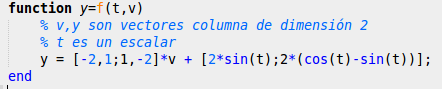
\includegraphics[width=\textwidth]{img/f.png}
    \end{minipage}
    \begin{minipage}{.4\textwidth}
        \centering
        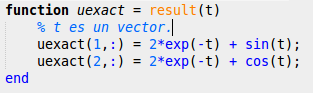
\includegraphics[width=\textwidth]{img/result.png}
    \end{minipage}
\end{center}

Una vez tenemos estas funciones definidas, procedemos a implementar el propio método de Euler, que podemos ver en la siguiente imagen.

\begin{center}
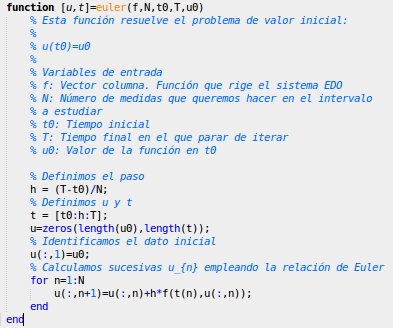
\includegraphics[width=0.6\textwidth]{img/euler.png}
\end{center}

Por último sólo tenemos que crear un programa principal que, llamando a las funciones ya definidas, resuelva el PVI planteado al inicio de esta sección.

\begin{center}
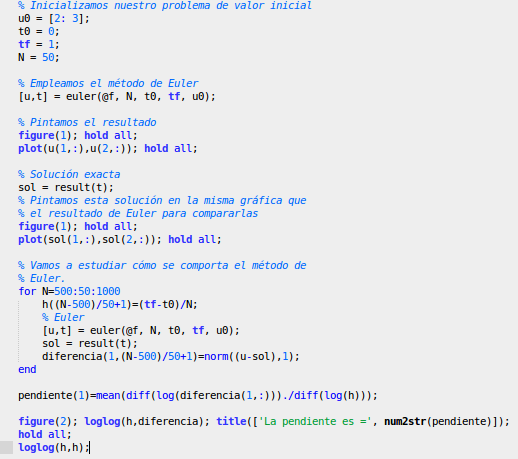
\includegraphics[width=0.8\textwidth]{img/aplicacion_euler.png}
\end{center}

Vamos a explicar detenidamente qué se está haciendo en este código. Para empezar estamos simplemente resolviendo el problema aplicando el método de Euler y pintando, en una misma gráfica, la solución dada por el método y la solución real, con lo que podemos observar la gran precisión de la solución obtenida por este método.
\begin{center}
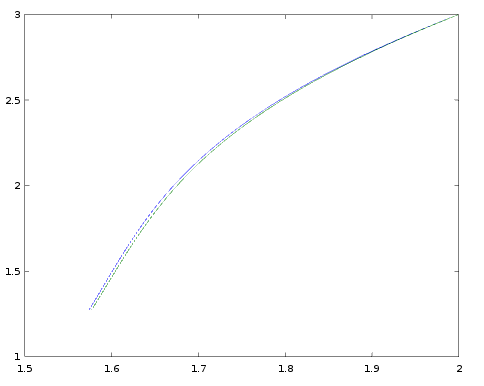
\includegraphics[width=0.8\textwidth]{img/figure1.png}
\end{center}

La última parte del código es la más compleja. Lo qye se está haciendo ahí es llamar numerosas veces al método de Euler y guardar, en cada llamada, la diferencia entre la función obtenida y la solución así como el $h$ empleado en esa ocasión.

Posteriormente calculamos la pendiente de la función que representan los pares de valores que hemos guardado. Para ello tomamos escala logarítmica y estudiamos la pendiente de la función en cada punto para, finalmente, tomar la media de esos valores.

Por último, pintamos estos valores junto con una función claramente lineal, que es $h$ con respecto a $h$ y obtenemos la siguiente gráfica.

\begin{center}
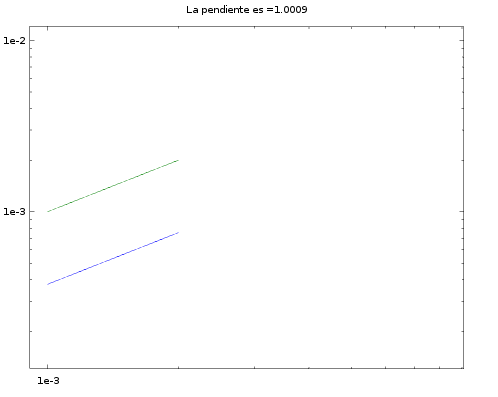
\includegraphics[width=0.8\textwidth]{img/figure2.png}
\end{center}

Ahora la pregunta que nos surge es clara, \textbf{¿por qué es interesante esta pendiente?}.

La idea se basa en el hecho de haber trabajado con logaritmos de los valores y no con los valores directamente. En general sabemos que el error se comporta como $e \leq c h^p$ para una cierta constante $c$, donde $p$ es el orden del método. Evidentemente podemos aplicar logaritmos a ambos lados sin que nada se estropee, obteniendo:
\[\log(e) \leq p \log(ch)\]

Si ahora dibujásemos la gráfica que relaciona el logaritmo del error con el logaritmo de $h$ obtendremos una recta con pendiente $p$ que es justo el \textbf{orden del método}.

Por tanto, esa pendiente que hemos calculado en el código, nos permite conocer el orden del método de Euler.

\section{Sesión 2}
\subsection{Método Runge Kutta de orden 4}
\subsubsection{Explícito}
En esta sesión vamos a implementar un método Runge Kutta explícito. Para ello, recordemos que el método Runge Kutta se basaba en el empleo de las funciones:
\[K_i = f(x_n+c_ih,y_n+\sum_j A_{ij}K_j)\]

En el caso del método Runge Kutta de cuarto orden teníamos:

\[
\begin{array}{ll}
K_1 = & f(x_n,y_n)\\
K_2 = & f(x_n+\frac{h}{2}, y_n+\frac{h}{2}K_1)\\
K_3 = & f(x_n+\frac{h}{2}, y_n + \frac{h}{2}K_2)\\
K_4 = & f(x_n+h, y_n + h K_3)
\end{array}
\]

Si escribimos todas las variables en una tabla (que sería la matriz de las $A_{ij}$ unida a la columna formada por las $c_i$) podemos ver que el método que origina la tabla es explícito si y sólo si no hay ningún elemento no nulo por encima de la diagonal principal.

\obs Queda como ejercicio para el lector la comprobación y el autoconvencimiento de que la afirmación anterior es cierta, pues es algo completamente trivial.

Para implementar el método, lo primero que hacemos es crear un fichero con la función \textit{PKexplicito} cuyo contenido se muestra a continuación
\begin{center}
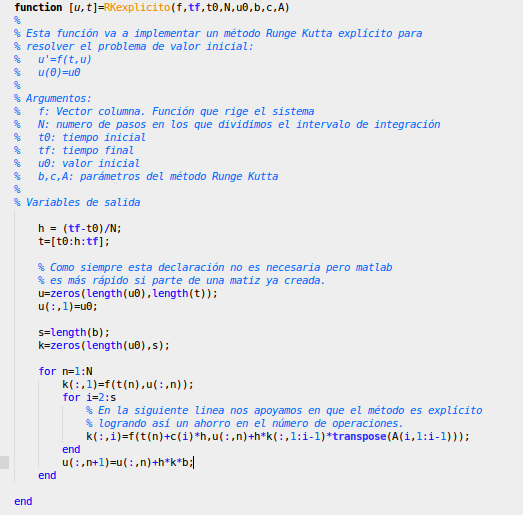
\includegraphics[width=0.6\textwidth]{img/RK4_explicito.png}
\end{center}

Ahora escribimos un pequeño programa que inicializará \textbf{el mismo PVI que ya resolvimos en la sesión de laboratorio anterior} (emplearemos por tanto las mismas funciones $f$ y $result$).
\begin{center}
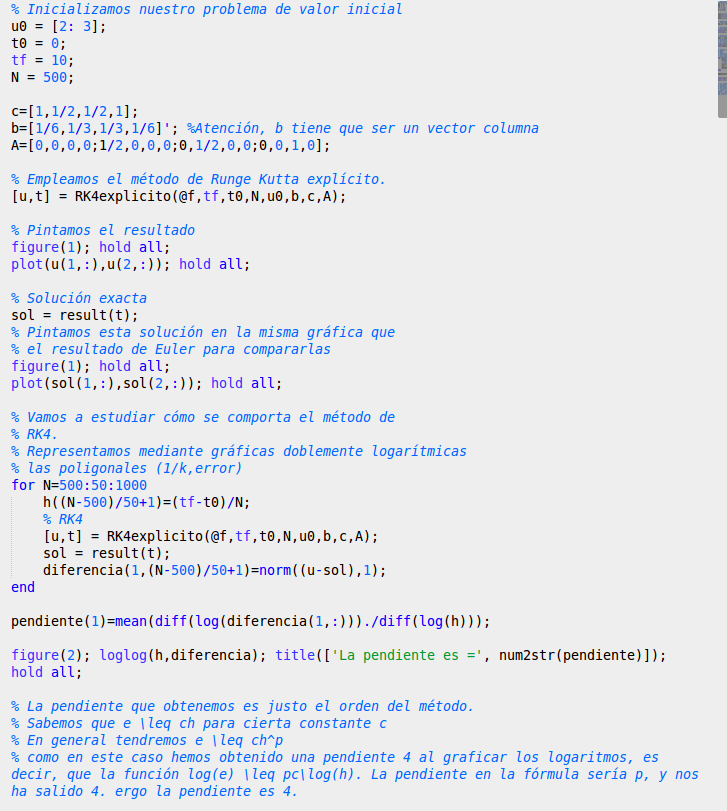
\includegraphics[width=0.6\textwidth]{img/PVI_RK4_explicito.png}
\end{center}

El código es totalmente equivalente al empleado en la sesión anterior, salvo que invocamos el método RK4 en lugar del método de Euler.

Las gráficas obtenidas, que dibujan la función resultado y la obtenida con RK4 por un lado y la relación entre el erro y $h$ en escala logarítmica por otro, son:
\begin{center}
    \begin{minipage}{0.49\textwidth}
        \centering
        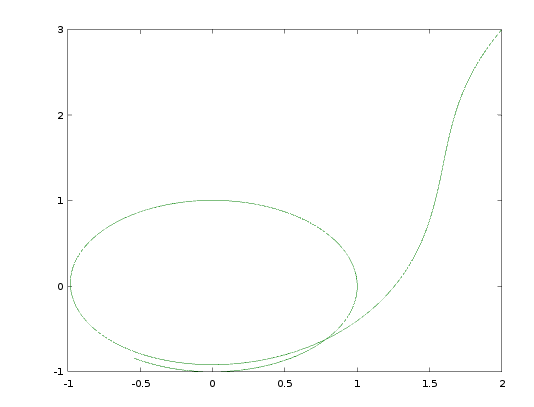
\includegraphics[width=\textwidth]{img/RK4_explicito_grafica.png}
    \end{minipage}
    \begin{minipage}{.49\textwidth}
        \centering
        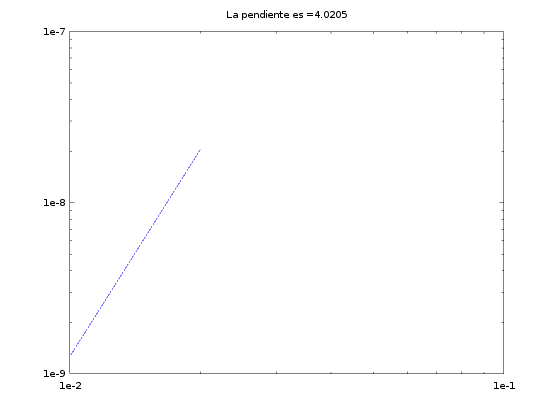
\includegraphics[width=\textwidth]{img/RK4_explicito_pendiente.png}
    \end{minipage}
\end{center}

Y tal y como hemos visto en clase, obtenemos que el método RK4 tiene orden 4.

\obs La diferencia observada entre esta función y la obtenida en la sesión anterior radica en el intervalo sobre el que estamos trabajando. En la ocasión anterior trabajamos en [0,1]; esta vez, en [0,10].

\subsubsection{Implícito}
Respecto a la sección anterior solo debemos modificar dos ficheros.

El fichero en que se define el problema de valor inicial pasara de llamarse \textit{PVI\_RK4\_explicito.m} a \textit{PVI\_RK4\_implicito.m}. Por otor lado, el fichero que contiene el propio método pasará a llamarse \textit{RK4implicito.m}. 

Veamos ahora cómo quedan estos dos nuevos ficheros.

La implementación del PVI queda igual salvo que modificamos la matriz A, para que tenga una diagonal no nula (en nuestro caso hemos puesto la diagonal llena de 1s), y modificamos las llamadas al método. 

La idea del método es que no conocemos las $K_i$ en un principio pero todas son, o pueden ser, necesarias para cada una de las demás $K_i$. 

Por tanto, lo que haremos será tratar de resolver un sistema de ecuaciones con el método del punto fijo. Así definimos para todos los $K_i$ un valor inicial, que será $f(x_n,y_n)$, y a partir de ahí iteramos encontrando en cada iteración toda una nueva serie de valores de los $K_i$.

En cada iteración empleamos todos los valores de $K_i$ de la iteración anterior y los actualizamos \textbf{todos ellos} al finalizar la iteración.

En algún momento esta iteración convergerá y tendremos los $K_i$ buscados.
Este fichero nos queda:

\begin{center}
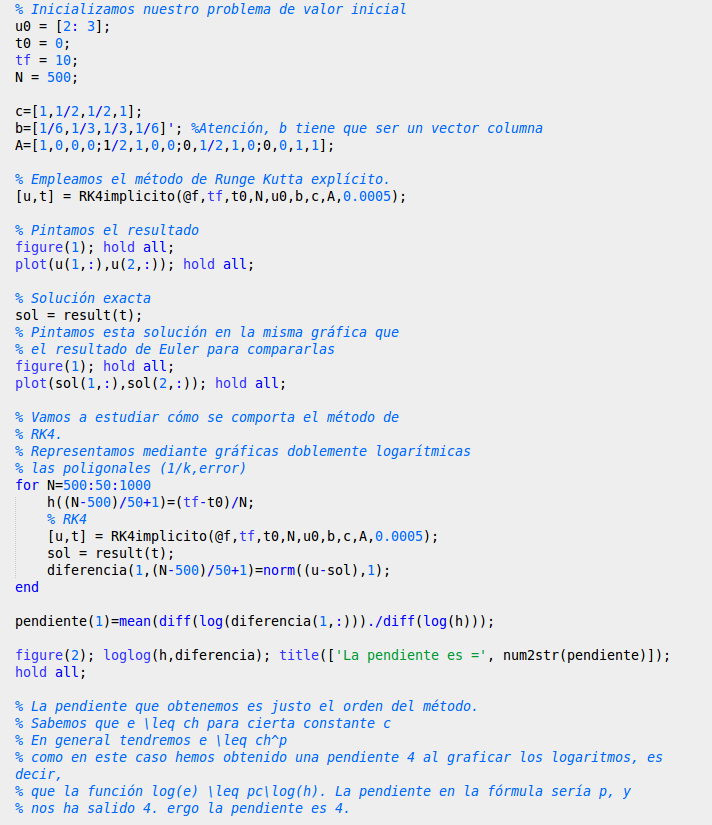
\includegraphics[width=0.6\textwidth]{img/PVI_RK4_implicito.png}
\end{center}

Y el propio método queda como sigue:
\begin{center}
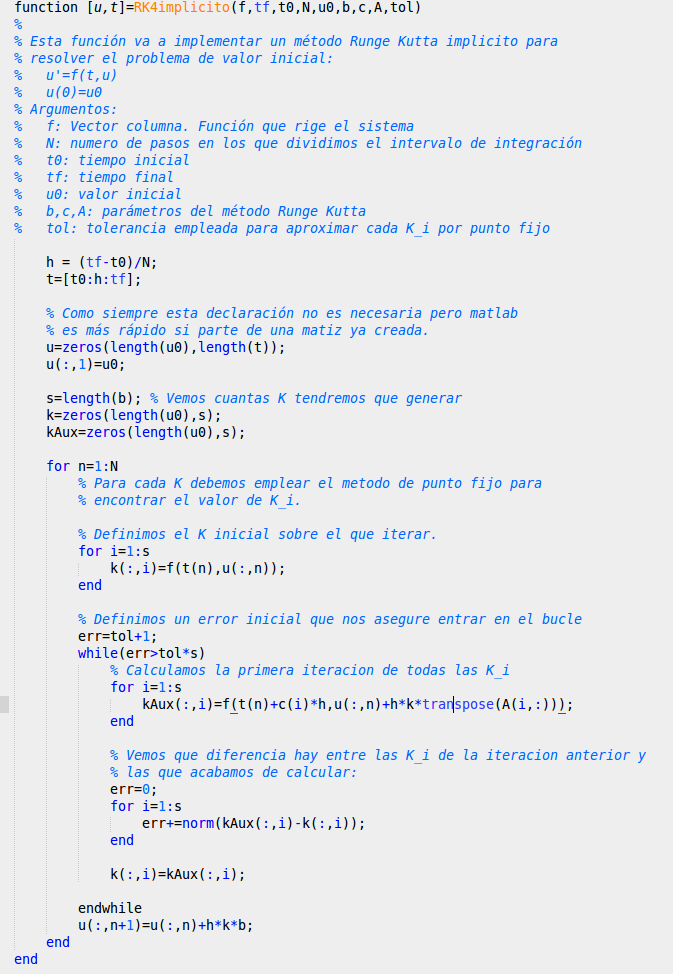
\includegraphics[width=0.6\textwidth]{img/RK4_implicito.png}
\end{center}

Finalmente, las gráficas obtenidas, que dibujan la función resultado y la obtenida con RK4 por un lado y la relación entre el erro y $h$ en escala logarítmica por otro, son:
\begin{center}
    \begin{minipage}{0.49\textwidth}
        \centering
        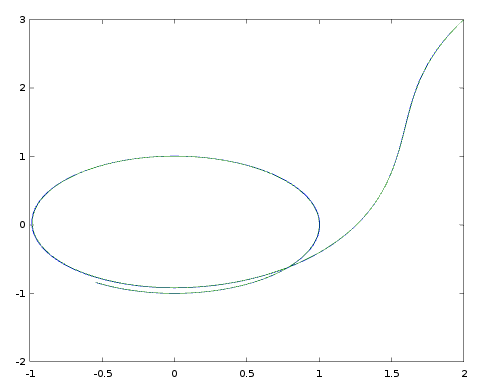
\includegraphics[width=\textwidth]{img/RK4_implicito_grafica.png}
    \end{minipage}
    \begin{minipage}{.49\textwidth}
        \centering
        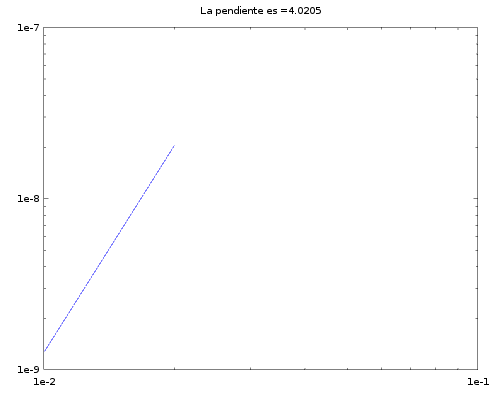
\includegraphics[width=\textwidth]{img/RK4_implicito_pendiente.png}
    \end{minipage}
\end{center}


\subsection{Método del trapecio}
Vamos a resolver una vez más el mismo PVI pero empleando esta vez el método del trapecio.

Para ello empezamos escribiendo una función que implemente dicho método:
\begin{center}
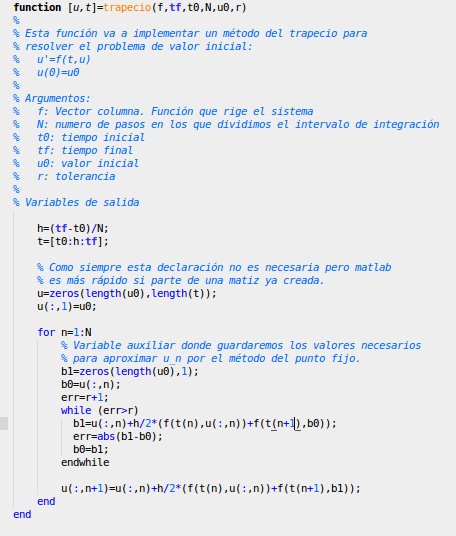
\includegraphics[width=0.6\textwidth]{img/trapecio.png}
\end{center}

La parte interesante de esta función se encuentra en el bucle while. El inconveniente del método del trapecio es que no es explícito, es decir, para calcular un $y_{n}$, la fórmula implica que necesitamos $y_n$.

La forma de resolver esto es aplicar el método del punto fijo para obtener una aproximación de $y_n$ y, a partir de esta aproximación, calcular el $y_n$ que nos da el método del trapecio.

Una vez tenemos el método implementado, reutilizamos las funciones $f$ y $resulto$ ya empleadas anteriormente y escribimos un pequeño programa que plantea el problema y lo resuelve incovando al método del trapecio.

\begin{center}
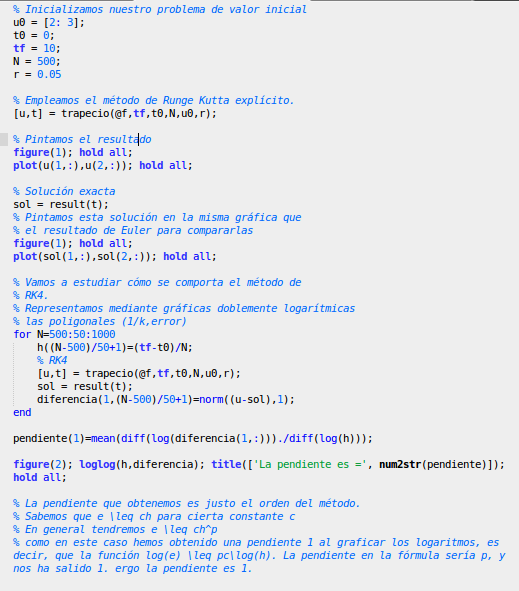
\includegraphics[width=0.6\textwidth]{img/PVI_trapecio.png}
\end{center}

Nuevamente, pintamos las gráficas de las funciones (la solución y la obtenida por el método numérico) para comprobar que coinciden y representamos el error respecto a $h$ en escala logarítmica para conocer la pendiente.

\begin{center}
    \begin{minipage}{0.49\textwidth}
        \centering
        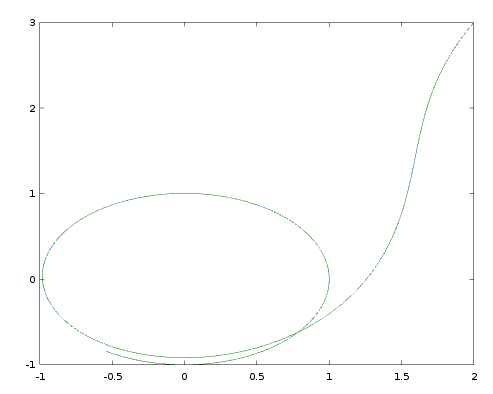
\includegraphics[width=\textwidth]{img/trapecio_grafica.png}
    \end{minipage}
    \begin{minipage}{.49\textwidth}
        \centering
        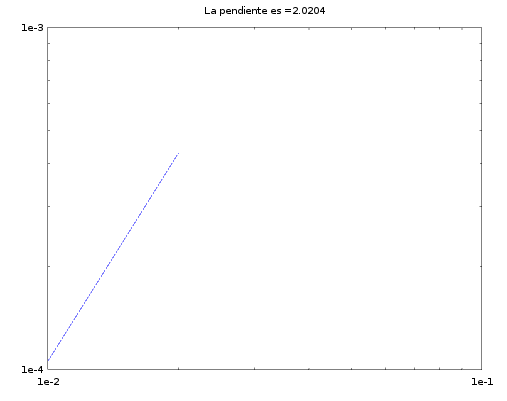
\includegraphics[width=\textwidth]{img/trapecio_pendiente.png}
    \end{minipage}
\end{center}


\appendix

\chapter{Ejercicios}
% -*- root: ../mnedo.tex -*-
\section{Hoja 1}
\begin{problem}[1]
Considerar el PVI:
\[\left\{ \begin{array}{l}y'=f(t) \ t \in [t_0,T] \\
y(t_0)=0\end{array}
\right.\]

Probar que utilizando el método de Euler:
\[y_N=\sum_{k=0}^{N-1} f(t_k)h\]
\solution

Recordamos que el método de Euler consiste en emplear
\[y_{n+1} = y_n + h f(t_n)\]

Por inducción podemos resolverlo:

\begin{equation*}
	\begin{multlined}[0.8\textwidth]
		\underline{n=0}: \quad y_1=y_0+h(t_0) = h(t_0)\\[1em]
		\shoveleft{\underline{n=1}: \quad y_2 = y_1 + hf(t_1) = hf(t_0) + hf(t_1)}\\
		\shoveleft{\qquad \qquad \quad = h\left[ f(t_0) + f(t_1) \right]}\\
	\end{multlined}
\end{equation*}

La hipótesis de inducción es que: $y_N = \sum_{k=0}^{N-1} f(t_k)h$. Así que solo nos falta demostrar que se cumple en $N+1$:
\[y_{N+1} = y_N + hf(t_N) = \sum_{k=0}^{N-1} f(t_k)h + hf(t_N) = \sum_{k=0}^N f(t_k)h\]

\end{problem}


\begin{problem}[2]
Ver que el método de Euler falla cuando queremos aproximar la solución
\[y(t) = t^{\frac{3}{2}}\]
del PVI
\[\left\{ \begin{array}{l}y'=\frac{3}{2}y^{\frac{1}{3}} \\
y(0)=0\end{array}
\right.\]

Justifica cuál es el problema.

\solution
\doneby{Pedro}

Recordamos que el método de Euler consiste en emplear
\[y_{n+1} = y_n + h f(y_n)\]

Puesto que el dato inicial es 0 y no hay ninguna constante positiva sumando en la $f(t_n,y_n)$, todas las $y_n$ que calculemos tendrán valor 0 con lo que el método no nos llevará a ningún sitio.

Si el método de Euler no nos lleva a ningún sitio, parece lógico pensar que la función debe tener algún problema que la hace salir del conjunto de funciones sobre las que se puede emplear este método.

Así parece lógico pensar que la función $f(t_n,y_n)=\frac{3}{2}y^{\frac{1}{3}}$ no es lipschitz en la segunda variable. Vamos a comprobarlo.

Sea $L$ la constante que define la condición de Lipchitz, siendo el intervalo en el que estamos trabajando el intervalo $[0, \infty)$. 

Tomamos en concreto $y_1=0$. En estas condiciones, si la función fuese Lipchitz tendríamos que 
\[\frac{\frac{3}{2}(y_2^{1/3})}{y_2} = \frac{3}{2}\frac{1}{y^{2/3}}\leq L y_2 \ \ \ \forall y_2 \in [0,\infty)\]

Llegados a este punto es sencillo ver que la parte de la izquierda tiende a infinito cuando $y_2$ tienda a 0 y por tanto no puede existir la constante $L$ que lo acote. Por tanto la función no es Lipchitz y no podemos aplicar el método de Euler.
\end{problem}

\begin{problem}[3]
Sea el PVI
\[\left\{ \begin{array}{l}y'=1+y^2 \ t \in [0,2] \\
y(0)=0\end{array}
\right.\]

¿Podemos usar el método de Euler para aproximar la solución $y(t)=\tan(t)$?

\solution

\doneby{Pedro}

Para empezar debemos de comprobar si la función que queremos aproximar satisface la ecuación planteada en el PVI.

\[\tan(x)' = \sec(x)^2 = 1 + \tan(x)^2, \ \ \tan(0)=0\]

Queda claro que el PVI planteado tiene como solución la función tangente. Ahora tenemos que ver si el problema planteado puede resolverse por el método de Euler.

Para verlo debemos comprobar si la función $f(t_n,y_n)=1+y^2$ es lipschitz en la segunda variable. Sólo en caso de serlo podríamos aplicar el método de Euler para obtener la solución. Vamos a ello.

\[\forall y_1<y_2 \in [0,2] \ \ \frac{\abs{y_2^2 - y_1^2}}{y_2-y_1}=\frac{(y_2-y_1)(y_2+y_1)}{y_2-y_1} = (y_2+y_1) \leq 4\]

Por tanto, como la función es Lipschitz en la segunda variable, podremos aplicar le método de Euler para resolver el PVI planteado.
\end{problem}


\begin{problem}[4]
Calcular el residuo de los siguientes métodos:

\ppart Regla del trapecio:
\[y_{n+1} = y_n + \frac{h}{2}\left( f(t_{n+1},y_{n+1})+f(t_n,y_n)\right)\]

\ppart Euler modificado:
\[y_{n+1} = y_n +hf\left( t_n+\frac{h}{2}, y_n+\frac{h}{2}f(t_n,y_n)\right)\]

\ppart Leap-frog
\[y_{n+2}=y_n+2hf(t_{n+1},y_{n+1})\]
\solution

\doneby{Pedro}

El residuo no es más que la diferencia entre el valor real de la función en $x_n$ y su valor aproximado a partir del método, es decir:
\[R_n = y(x_{n+1})-y_{n+1}\]

\spart
\[R_n = y(x_{n+1})-y_{n+1} = y(x_{n+1})-y(x_n) - \frac{h}{2}\left( y'(x_{n+1})+y'(x_n)\right)\]

Por Taylor podemos ver que:
\[\left\{\begin{array}{l}
y(x_{n+1}) = y(x_n)+hy'(x_n)+\frac{h^2}{2}y''(x_n)+O(h^3) \\
y'(x_{n+1}) = y'(x_n)+hy''(x_n) +O(h^2)
\end{array}\right.\]

Sustituyendo estos datos en la fórmula del residuo llegamos a:
\[R_n = O(h^3)\]

Puesto que el orden del método viene dado por $\frac{R_n}{h}$, en esta ocasión tenemos que el método del trapecio tiene un orden de consistencia al menos $2$.

Si realizásemos los desarrollos de Taylor con un orden mayor veríamos que el residuo deja de poder expresarse como $O(h^i)$, es decir, deja de estar controlado por $h$ con lo que podemos confirmar que el orden de consistencia del método es 2.

\spart

En esta ocasión
\[R_n = y(x_{n+1})-y(x_n)-hf\left( t_n+\frac{h}{2}, y_n+\frac{h}{2}y'(x_n)\right)\]

Calculando el desarrollo de Taylor de la $f$ llegamos a:
\[f\left( t_n+\frac{h}{2}, y_n+\frac{h}{2}y'(x_n)\right) = f(x_n,y_n)+\frac{h}{2}f_x(x_n,y_n)+\frac{h}{2}y'(x_n)f_y(x_n,y_n)= \atop y'(x_n)+\frac{h}{2}y''(x_n)+O(h^2)\]

Sustituyendo en la fórmula del residuo llegamos a:
\[R_n = O(h^3)\]

Si encomendamos nuestro alma al diablo y tratamos de estudiar si el residuo es de orden 3 vemos que no lo es, con lo que queda claro que el residuo es de orden 3 y por tanto el método es consistente de orden 2.

\spart

En esta ocasión
\[R_n = y(x_{n+2})-y(x_n)-2hy'(x_{n+1})\]

Desarrollando por Taylor el primer sumando tenemos 
\[\left\{ \begin{array}{l}
y(x_{n+2}) = y(x_n) + 2hy'(x_n)+2h^2y''(x_n)+O(h^3) \\
y'(x_{n+1}) = y'(x_n)+hy''(x_n) + O(h^2)
\end{array}\right.\]

Y sustituyendo en la fórmula del residuo llegamos a:
\[R_n=O(h^3)\]


\end{problem}

\begin{problem}[5]
Dado $α \in [0,1]$ encontrar el orden del método:
\[y_{n+1} = y_n +hf(t_n+(1-α)h, αy_n+(1-α)y_{n+1})\]

\solution

Lo que debemos hacer es calcular el residuo cuya definición, recordemos, era:

\begin{defn}[Residuo]
Cuánto de lejos está la solución de satisfacer en un paso la fórmula de recurrencia
\end{defn}

Según esta definición, nuestro residuo será:
\[R_n = \underbrace{y(t_{t+1})}_{\label{ej1-5_tresTerminos}1} - \left\{ \underbrace{y(t_n)}_{2} + \underbrace{hf(t_n+(1-α)h, αy(t_n)+(1-α)y(t_{n+1}))}_{3} \right\}\]

Para conocer el orden de este residuo nos serviremos de los desarrollos de Taylor:
\[\hyperref[ej1-5_tresTerminos]{1} \quad y(t_{n+1}) = y(t_n)+y'(t_n)h + y''(t_n)\frac{h^2}{2} + O(h^3)\]

La segunda variable para la $f$ que aparece en \hyperref[ej1-5_tresTerminos]{3} se puede desarrollar como:
\[αy(t_n) + (1-α)y(t_{n+1}) = αy(t_n) + (1-α)\left[y(t_n) + y'(t_n)h +  y''(t_n)\frac{h^2}{2} + O(h^3) \right] \]
\[\qquad \qquad \qquad \qquad = y(t_n) + (1-α)\left[ y'(t_n)h + y''(t_n) \frac{h^2}{2} + O(h^3) \right]\]

Por tanto el desarrollo de Taylor de \hyperref[ej1-5_tresTerminos]{3} puede expresarse de la siguiente forma:

\[h\left( f(t_n,y(t_n))+\underbrace{f_x(t_n,y(t_n))\cdot (1-α)h +\underbrace{f_y(t_n,y(t_n))(1-α)h\left( y'(t_n)+y''(t_n)\frac{h}{2}+O(h^3)\right)}_{f_y(t_n,y(t_n))y'(t_n)(1-α)h + O(h^2)}}_{(1-α)h y''(t_n) + O(h^2)}\right) = \]

\[=hy'(t_n)+(1-α)h^2y''(t_n)+O(h^3)\]

De modo que las 3 expresiones las tenemos como:
\begin{equation*}
	\begin{multlined}[.8\textwidth]
		\hyperref[ej1-5_tresTerminos]{1} =  \quad y(t_{n+1}) = y(t_n) + y'(t_n) h + y''(t_n) \frac{h^2}{2} + O(h^3) \\
		\shoveleft{\hyperref[ej1-5_tresTerminos]{2} =  \quad y(t_n)} \\
		\shoveleft{\hyperref[ej1-5_tresTerminos]{2} =  \quad hy'(t_n) + (1-α) h^2 y''(t_n) + O(h^3)}\\
	\end{multlined}
\end{equation*}


Sumando \hyperref[ej1-5_tresTerminos]{1} y \hyperref[ej1-5_tresTerminos]{3}, y restando \hyperref[ej1-5_tresTerminos]{2} obtenemos:
\[R_n = y''(t_n)h^2 \left(\frac{1}{2}-(1-α) \right)+O(h^3)\]


Ahora tenemos dos casos posibles, y sabiendo que el orden de un método es $\frac{R_n}{h}$:
\begin{itemize}
\item α=1/2
\[R_n=O(h^3) \implies \text{ orden } \geq 2\]
\item α$\neq$1/2
\[R_n = y''(t_n)h^2 \left(\frac{1}{2}-(1-α) \right) + O(h^3) \implies \text{ orden } 1\]
\end{itemize}

\end{problem}


\begin{problem}[6]
	\ppart Sea un PVI. Utilizando los polinomios de interpolación de Lagrange obtener el método de Adams-Bashforth de dos pasos
	\[y_{n+2} = y_{n+1} + h \left( \frac{3}{2}f(t_{n+1}, y_{n+1}) + \frac{1}{2}f(t_n,y_n) \right),\]
	
	\ppart y el de tres pasos
	\[y_{n+3} = y_{n+2} + h \left( \frac{23}{12} f(t_{n+2},y_{n+2}) - \frac{4}{3} f(t_{n+1}, y_{n+1}) + \frac{5}{12}f(t_n,y_n) \right)\]
	
	\solution
	\begin{defn}{\textbf{Polinomio de interpolación de Lagrange}}

		Recordemos (de cálculo numérico) que el polinomio de interpolación de Lagrange tenía la forma:
		\[P(x) = f(x_0)l_0(x) + f(x_1)l_1(x) + … + f(x_N)l_N(x)\]
		donde $f$ es la función que queremos aproximar en los $x_i,\ i=0,…,N$ puntos, y
		\[l_i(x) = \frac{(x-x_0) … (x-x_{i-1}) (x-x_{i+1}) … (x-x_N)}{(x_i-x_0) … (x_i-x_{i-1}) (x_i-x_{i+1}) … (x_i-x_N)}\]
	\end{defn}

	\spart
	En el método de Adams Bashforth tenemos que
	\[y(x_{n+2})-y(x_{n+1}) = \int_{x_{n+1}}^{x_{n+2}} f(x,y(x)) dx\]
	y el valor de $f$ entre los puntos $x_{n+1}, x_{n+2}$ se aproximama mediante la recta que pasa por los puntos $(x_{n+1},f(x_{n+1},y_{n+1}), (x_{n+2}, f(x_{n+2},y_{n+2})))$. Para obtener dicha recta usamos el polinomio de interpolação de Lagrange:
	\[f(x,y) = f(x_n,y_n)\frac{x-x_{n+1}}{x_n-x_{n+1}} + f(x_{n+1},y_{n+1}) \frac{x-x_n}{x_{n+1}-x_n}\]

	Si integramos entre $\int_{x_{n+1}}^{x_{n+2}}$
	\[\int_{x_{n+1}}^{x_{n+2}} \left[ f(x_n,y_n)\frac{x_{n+1}-x}{h} + f(x_{n+1},y_{n+1})\frac{x-x_n}{h} \right]dx =\]
	\[= \left[ f(x_{n+1},y_{n+1}) \frac{(x-x_n)^2}{2h} - f(x_n,y_n)\frac{(x_{n+1}-x)^2}{2h} \right]_{x_{n+1}}^{x_{n+2}}  =\]
	\[= \frac{1}{2h}f(x_{n+1},y_{n+1}) \left[ (x_{n+2}-x_n)^2 - (x_{n+1}-x_n)^2 \right] - \frac{1}{2h} \left[ (x_{n+1} - x_{n+2})^2 - (x_{n+1} - x_{n+1})^2 \right] =\]
	\[= \frac{h}{2} \left( 3f(x_{n+1},y_{n+1}) - f(x_n,y_n) \right)\]


	\spart
	En este caso tendremos que:
	\[y_{n+1} - y_n = \int_{x_n}^{x_{n+1}} f(x,y(x)) dx\]
	Con la particularidad de que ahora la aproximación de $f$ en el intervalo $[x_n,x_{n+1}]$ la realizaremos interpolando la $f$ en los puntos $x_{n-2},x_{n-1},x_n$ con el polinomio de Lagrange $p$.

	Sabemos por tanto que $p$ interpola $f$ en $x_{n-2},x_{n-1},x_n$:

	\begin{center}
	\inputtikz{EJRC_interpolar}
	\end{center}

	Para simplificar los cálculos vamos a tomar el cambio de variable $u=\frac{x_{n+1}-x}{h}$ para que así el polinomio interpole $f(u,y(u))$ en los puntos $3,2,1$. ($u(x_{n-2})=3, u(x_{n-1})=2, u(x_n)=1$).

	\begin{center}
	\inputtikz{EJRC_interpolar_transformed}
	\end{center}


	Es decir, tras el cambio de variable el polinomio interpolador queda como

	\[\tilde{p}(u) = f(x_n,y_n) \frac{(u-2)(u-3)}{(1-2)(1-3)} + f(x_{n-1},y_{n-1}) \frac{(u-1)(u-3)}{(2-1)(2-3)}+f(x_{n-2},y_{n-2}) \frac{(u-1)(u-2)}{(3-1)(3-2)}\]

	De modo que tras el cambio de variable tendremos:
	\[\int_{x_n}^{x_{n+1}}p(x)dx \underbrace{=}_{t_{n+1}-hu=x} h\int_0^1 p(t_{n+1}-hu) du = h\int_0^1 \tilde{p}(u)du =\]
	\[= h\int_0^1 \left[ f(x_n,y_n) \frac{(u-2)(u-3)}{(1-2)(1-3)} + f(x_{n-1},y_{n-1}) \frac{(u-1)(u-3)}{(2-1)(2-3)}+f(x_{n-2},y_{n-2}) \frac{(u-1)(u-2)}{(3-1)(3-2)} \right] =\]
	\[= h\int_0^1 \left[ f(x_n,y_n)\frac{u^2-5u+6}{2} - f(x_{n-1},y_{n-1})(u^2-4u+3) + f(x_{n-2},y_{n-2})\frac{u^2-3u+2}{2} \right] =\]
	\[=  h \left( \frac{23}{12} f(t_{n+2},y_{n+2}) - \frac{4}{3} f(t_{n+1}, y_{n+1}) + \frac{5}{12}f(t_n,y_n) \right)\]

	Por tanto
	\[y(x_{n+2})-y(x_{n+1}) = \int_{x_{n+1}}^{x_{n+2}} p(x) dx = h \left( \frac{23}{12} f(t_{n+2},y_{n+2}) - \frac{4}{3} f(t_{n+1}, y_{n+1}) + \frac{5}{12}f(t_n,y_n) \right)\]
\end{problem}

\begin{problem}[7]
La regla de integración del trapecio se define por:

\[y_{n+1} = y_n + \frac{h}{2}\left( f(t_{n+1},y_{n+1})+f(t_n,y_n)\right)\]

Probar que la regla del trapecio es 0-estable. Nótese que basta con demostrar que la función incremento asociada a esta regla, $\phi(t,y;h)$ cumple:
\begin{enumerate}
\item Es continua con respecto a las variables $t,y,h$
\item Es Lipschitz con respecto a la variable $y$
\item Si $f=0$, entonces $\phi_f=0$
\end{enumerate}
\solution

\doneby{Pedro}

Técnicamente el ejercicio está hecho en clase pero yo me preocupé de copiarlo aquí de nuevo.

\begin{itemize}
\item Es continua con respecto a las variables $t,y,h$

Definimos la aplicación global contractiva
\[F(\phi) = \frac{1}{2} \left[ f(x_n,y_n) + f(x_{n+1}, y_n+h\phi) \right]\]

Y tomamos $\phi_f = \lim_{j\to∞} \phi_f^{[j]}$, donde $\phi_f^{[j]}$ viene dada por la sucesión $\phi_f^{[j]} = F\left(\phi_f^{[j-1]}\right)$ y $\phi^0 = 0$.

\obs El método del trapecio es de 1 paso ($k=1$) y por tanto la función incremento solo depende de $x_n$, $y_n$ y $h$, es decir $\phi_f(x_n,y_n;h)$.

Dado que $f$ es una función continua, tendremos que la función:
\[\phi_f^{[1]}(x_n,y_n;h) = \frac{1}{2} \left[ f(x_n,y_n) + f(x_{n+1}, y_{n+1} + 0) \right]\]
será continua. Como la composición de funciones continuas da como resultado otra función continua, tendremos que $\phi_f^{[2]}=F\left( \phi_f^{[1]} \right)$ es continua, y por tanto todas las $\phi_f^{[k]}(x_n,y_n;h)$ son continuas.

Si logramos probar que la convergencia de las $\phi_f^{[j]}$ sea uniforme, tendremos que la sucesión convergería a una función $\phi_f$ continua.

Expresamos $\phi_f^{[k]}$ como una suma telescópica:
\begin{equation}
	\label{eq:suma_telesc_pto_fijo_ej}
	\phi_f^{[k]} = \sum_{j=1}^k \phi_f^{[j]} - \phi_f^{[j-1]} + \phi_f^{[0]},\quad \phi_f^{[0]}=0
\end{equation}
Tomando la norma $L^∞$:
\begin{equation*}
	\begin{multlined}[0.7\textwidth]
		\md{\phi_f^{[j]} - \phi_f^{[j-1]} }_{L^∞} = \md{F\left[\phi_f^{[j-1]}\right] - F\left[\phi_f^{[j-2]}\right] }_{L^∞}\\[1em]
		\shoveleft{\qquad \qquad \qquad \underbrace{≤}_{F\text{ contractiva}} \frac{Lh}{2} \md{\phi_f^{[j-1]} - \phi_f^{[j-2]}}_{L^∞}}\\
	\end{multlined}
\end{equation*}
Aplicando la desigualdad sucesivamente:
\[\md{\phi_f^{[j]} - \phi_f^{[j-1]}}_{L^∞} ≤ \left(\frac{Lh}{2}\right)^{j-1} \md{\phi^{[1]}}_{L^∞}\]

Puesto que $K = [a,b]×ℝ×(0,∞)$ es compacto:
\[\md{\phi_f^{[j]} - \phi_f^{[j-1]}}_{L^∞} ≤ M_k\left(\frac{Lh}{2}\right)^{j-1}\]

De modo que aplicando el test $M$ de Weierstrass, la convergencia de \ref{eq:suma_telesc_pto_fijo_ej} es uniforme, y por tanto $\phi_f$ es continua.

\item Es Lipschitz con respecto a la variable $y$

%En el apartado anterior hemos visto que podemos construir una sucesión de funciones que converge uniformemente a $\phi_f$. Todas estas funciones seran funciones Lipschitz con respecto a la $y$ (que es la segunda variable de $\phi_f$) y por tanto todas las $\phi_f^{[j]}$ son Lipschitz.

%Puesto que la convergencia es uniforme, el límite también es una función Lipschitz. 

%Vamos a demostrar esta afirmación para los lectores incrédulos.
%\begin{proof}
%De forma general vamos a considerar una sucesión de funciones $f_x(x,y)$ que converge uniformemente a $f(x,y)$. 

%Por definición de convergencia uniforme, tenemos:
%\[\forall ε > 0 \exists n \tq \forall N > n \ \ \norm{f(x,y)-f_n(x,y)} \leq ε\]

%Vamos a estudiar ahora la ``Lipschitzialidad'' de la función $f$ sabiendo que todas las $f_n$ son Lipschitz.

%\[\norm{f(x,y)-f(x,y')} = \norm{f(x,y)\pm f_n(x,y)\pm f_n(x,y')+f(x,y')} \leq \]
%por la desigualdad triangular
%\[\leq \norm{f(x,y)-f_n(x,y)}+\norm{f(x,y')-f_n(x,y')}+\norm{f_n(x,y)-f_n(x,y')} = \atop 2ε +\norm{f_n(x,y)-f_n(x,y')}\]

%Finalmente, puesto que las $f_n$ son Lipschitz tenemos que:
%\[2ε +\norm{f_n(x,y)-f_n(x,y')} \leq 2ε + \norm{y-y'}\]

%Puesto que $\forall ε > 0$ podemos encontrar un $n$ que nos permita llevar a cabo estas operaciones, podemos hacer ε tan pequeño como queramos y llegar a:
%\[\norm{f(x,y)-f(x,y')} \leq \norm{y-y'}\]
%\end{proof}
Por definición, para el método del trapecio tenemos que $\phi_f$ es la solución de
\[\phi_f (x_n,y_n) = \frac{h}{2}\left(f(x_n,y_n)+f(x_{n+1},y_{n+1}) \right) = \frac{1}{2}\left( f(x_n,y_n) + f(x_{n+1},y_n+h\phi_f(x_n,y_n)\right)\]

Con la definición de $\phi_f$ podemos escribir
\[\norm{\phi_f(x_n,y_n,h)-\phi_f(x_n,\tilde{y}_n,h)}  \leq \]
\[\leq \frac{1}{2}\norm{f(x_n,y_n)-f(x_n,\tilde{y}_n)}+\frac{1}{2}\norm{f(x_{n+1},y_n+h\phi_f(x_n,y_n))-f(x_{n+1},\tilde{y}_n+h\phi_f(x_n,\tilde{y}_n))} \leq\footnote{por ser $f$ Lipschitz}\]
\[\leq L\norm{y_n-\tilde{y}_n}+\frac{Lh}{2}\norm{\phi_f(x_n,y_n,h)-\phi_f(x_n,\tilde{y}_n,h)}\]

Reordenando los términos de la inecuación podemos escribir:
\[\left(1-\frac{Lh}{2} \right)\norm{\phi_f(x_n,y_n,h)-\phi_f(x_n,\tilde{y}_n,h)} \leq L\norm{y_n-\tilde{y}_n}\]
\item Si $f=0$, entonces $\phi_f=0$

Puesto que en el método del trapecio $\phi_f$ se define como el punto fijo de
\[F(\phi) = \frac{1}{2} \left[ f(x_n,y_n) + f(x_{n+1}, y_n+h\phi) \right]\]

si $f=0$ tendremos que $\phi_f$ será el punto fijo de la función nula y, por tanto, será 0

\end{itemize}
\end{problem}

\begin{problem}[8]
Probar que los métodos de Adams-Bashforth de dos pasos y de tres pasos, definidos en el ejercicio 6, son convergentes.
\solution
\doneby{Jorge}

En este ejercicio primero probaremos que los métodos son consistentes usando el teorema \ref{theorem:consist_iif_relaciones}. Después probaremos que son 0-estables, y sirviéndonos del teorema \ref{theorem:consist_y_0estable_converge} podremos decir que el MN es convergente.

Este ejercicio lo hicimos antes de conocer el criterio de la raíz \ref{theorem:criterio_raiz}, que simplifica enormemente la demostración de la 0-estabilidad. Al final de cada apartado se encuentra la versión del profesor, que emplea este criterio.
\textcolor{red}{
\obs Para poder aplicar los teoremas vistos en clase sobre métodos numéricos, antes debemos comprobar que el método con el que trabajamos satisface las hipótesis de un buen método numérico y, por tanto, los teoremas son válidos.}

\spart \textbf{Método de 2 pasos}:

El método de Adams-Bashforth de dos pasos se trata de un método basado en cuadratura que emplea la relación
\[y(x_{n+2}) - y(x_{n+1}) = \int_{x_{n+1}}^{x_{n+2}} f(x,y(x)) \dif x\]

donde $f(x,y(x))$ se aproxima por medio de la recta interpolante entre los puntos $(x_n,y(x_n))$ y $(x_{n+1},y(x_{n+1}))$, es decir:
\[f(x,y(x)) \approx f(x_n, y(x_n)) \frac{x-x_{n+1}}{x_n-x_{n+1}}+f(x_{n+1},y(x_{n+1}))\frac{x-x_n}{x_{n+1}-x_n}\]

Finalmente, el método queda expresado como:
\[y_{n+2} = y_{n+1}+\frac{h}{2}\left( 3f(x_{n+1},y_{n+1})-f(x_n,y_n)\right)\]

\textbf{El ejercicio propiamente dicho empieza a partir de esta última igualdad, lo anterior sólo era para entrar en calor}

\begin{enumerate}
\item \textbf{Consistencia}

Es sencillo ver que \[\sum_{j=0}^{k=2} α_j = 0 - 1 + 1 = 0\]

Para este método, tenemos la función incremento
\[\phi_f(x_n,y_n,h) = \frac{1}{2}\left(3f(x_n+h,y_n+h\phi_f(x_n,y_n,h))-f(x_n,y_n)\right)\]

De donde podemos ver que:
\[\phi_f(x,y(x),0) = \frac{1}{2} \left(3f(x,y(x)) - f(x,y(x)) \right) = f(x,y(x))\]

Para poder aplicar el teorema \ref{theorem:consist_iif_relaciones} necesitamos ver que:
\[\phi_f(x,y(x),0)  = \sum_{j=0}^2jα_jf(x,y(x))=-f(x,y(x)) + 2 f(x,y(x)) = f(x,y(x))\]

Por tanto, podemos aplicar el teorema \ref{theorem:consist_iif_relaciones} y garantizar así que el método es consistente.

\item \textbf{0-estabilidad}

Consideramos dos sucesiones: $\left\{ y_n \right\}_{n=0}^N$, $\left\{ y(x_n) \right\}_{n=0}^N$ y buscamos las sucesiones $δ_n,γ_n$ asociadas, que serán aquellas que satisfagan las ecuaciones:

\[\sum_{j=0}^kα_jy_{n+j} = h\phi_f(x_n,y_n,...,y_{n+j},h)+hδ_n\]
\[\sum_{j=0}^kα_jy(x_{n+j}) = h\phi_f(x_n,y(x_n),...,y(x_{n+j}),h)+hγ_n\]

Para poder garantizar la 0-estabilidad, por definición, debemos probar que 
\[\max_{k \leq n \leq N}\norm{y_n - y(x_n)} \leq C\left( \max_{0 \leq n \leq k-1}\norm{y(x_n) - y_n}+\max_{0 \leq n \leq N-k}\norm{δ_n - γ_n}\right)\]

Por la propia definición del método numérico tenemos que $δ_n=0$. Vamos a estudiar la diferencia entre las sucesiones:

\[y(x_{n+2})-y_{n+2} = y(x_{n+2}) - y_{n+1} - \frac{h}{2}\left( 3f(x_{n+1},y_{n+1}) - f(x_n,y_n)\right)\]

Desarrollando con Taylor en torno a $x_n$ tenemos:
\[y(x_{n+2}) = y(x_n)+2hf(x_n,y(x_n))+O(h^2)\]
\[y_{n+1} = y_n +hf(x_n,y_n)+O(h^2)\]
\[f(x_{n+1},y_{n+1}) = y'_{n+1} = f(x_n,y_n) + O(h)\]

Sustituyendo en la diferencia tenemos:
\[y(x_{n+2})-y_{n+2} = y(x_n)-y_n+ h(2f(x_n,y(x_n))-f(x_n,y_n)) - hf(x_n,y_n)+ O(h^2) =\]
\[=y(x_n)-y_n+2h(f(x_n,y(x_n))-f(x_n,y_n)) + \underbrace{O(h^2)}_{\text{residuo = }hδ_n}\]

Ahora procedemos a acotar la diferencia:
\[\underbrace{\norm{y(x_{n+2})-y_{n+2}}}_{\max_{k \leq n \leq N}\norm{y_n - y(x_n)}} \leq \norm{y(x_n)-y_n} + 2hL\norm{y_n-y(x_n)}+hδ_n \leq \underbrace{(Kh)}_C\left(\underbrace{\norm{y_n-y(x_n)}}_{\max_{0 \leq n \leq k-1}\norm{y(x_n) - y_n}}+δ_n\right)\]

Con lo que vemos que, efectivamente, se cumple la condición de 0-estabilidad

\textbf{Versión del profesor}

Para estudiar la 0-estabilidad aplicamos el criterio de la raíz.

En esta ocasión el primer polinomio característico es $P(x)=x^2-x$, cuyas raíces son 0 y 1 con lo que, efectivamente se satisface el criterio de la raíz pues una raíz tiene módulo menor que 1 y la que tiene módulo 1 es simple.

\end{enumerate}

\spart \textbf{Método de 3 pasos}:

\begin{enumerate}
\item \textbf{Consistencia}

Se cumple la primera afirmación de la parte derecha de \ref{theorem:consist_iif_relaciones}:
\[\sum_{j=0}^{k=3} α_j = 1 - 1 + 0 + 0 = 0\]

En este caso $\phi_f(x_n,y_n,y_{n+1},y_{n+2}, h) = \frac{23}{12}f(x_n+2h, y_{n+2}) - \frac{16}{12}f(x_n+h,y_{n+1}) + \frac{5}{12}f(x_n,y_n)$, y por tanto se cumple la segunda afirmación de la parte derecha de \ref{theorem:consist_iif_relaciones}:
\[\phi_f(x,y(x),y(x),y(x), 0) = \frac{23}{12}f(x+2h, y(x)) - \frac{16}{12}f(x,y(x)) + \frac{5}{12}f(x,y(x)) = \overbrace{1}^{\sum_{j=0}^{k=3} jα_j} f(x,y(x))\]

\item \textbf{0-estabilidad}
Por tanto \textbf{el MN es 0-estable} y por tanto es consistente. Así que solo nos queda ver que el MN es 0-estable:

Tomamos las sucesiones $\left\{ y_n \right\}_{n=0}^N$, $\left\{ y(x_n) \right\}_{n=0}^N$ y las restamos:

\small
\begin{equation*}
	\begin{multlined}[\textwidth]
		y(x_{n+3}) - y_{n+3} = y(x_{n+2}) - y_{n+2} + h\frac{23}{12}\left(f(x_{n+2},y(x_{n+2})) - f(x_{n+2},y_{n+2})\right) + \\[1em]
		~
		\shoveleft{\qquad + h \left\{- \frac{16}{12}\left(f(x_{n+1},y(x_{n+1})) - f(x_{n+1},y_{n+1})\right) + h \frac{5}{12}\left(f(x_n,y(x_n)) - f(x_n,y_n)\right) \right\} + \overbrace{hδ_n}^{R_n}}\\
	\end{multlined}
\end{equation*}
\normalsize

Tomando valores absolutos a ambos lados y usando que $f$ es Lipschitz en la segunda variable:
\small
\begin{equation*}
	\begin{multlined}[\textwidth]
		\abs{y(x_{n+3}) - y_{n+3}} ≤ \\[1em]
		~
		\shoveleft{\qquad ≤ \abs{y(x_{n+2}) - y_{n+2}} + \frac{23}{12}Lh \left\{\abs{y(x_{n+2})-y_{n+2}} + \abs{y(x_{n+1})-y_{n+1}} + \abs{y(x_n)-y_n} \right\} + h\abs{δ_n} ≤}\\
		~
		\shoveleft{\qquad ≤ \left(1+\frac{23}{12}Lh\right) \left\{\abs{y(x_{n+2})-y_{n+2}} + \abs{y(x_{n+1})-y_{n+1}} + \abs{y(x_n)-y_n} + \abs{δ_n} \right\} ≤}\\
		\shoveleft{\qquad ≤ 3\left(1+\frac{23}{12}Lh\right) \left\{\max_{0≤j≤2}\abs{y(x_{n+j})-y_{n+j}} + \abs{δ_n} \right\}}\\
	\end{multlined}
\end{equation*}
\normalsize

Con lo que queda claro que el método es 0-estable

\textbf{Versión del profesor}

El primer polinomio característico es $P(x) = x^3-x^2$ que tiene como solución doble al 0 y como solución simple al 1, por lo que satisface el criterio de la raíz, lo que nos garantiza que el método es 0-estable.
\end{enumerate}

\end{problem}

\section{Problemas previos al primer parcial}

En esta sección incluimos todos los problemas realizados en clase a modo de preparación para el primer parcial, que no están incluidos en las hojas de ejercicios.

\begin{problem}[1]
Probar la convergencia del método de Euler sabiendo que es consistente:

\solution

Recordemos que el método de Euler es un método numérico que permite resolver un problemas de valor inicial mediante la recursión:
\[y_{n+1} = y_n + hf(x_,y_n)\]

Sabiendo esto, podemos ver que el residuo puede escribirse como:
\[y(x_{n+1}) = y(x_n) + hf(x_n,y_n) + R_n\]
que no es más que aplicar la definición de residuo.

Dado el dato inicial $y(0)=y^0$, para poder ver que el método es convergente debemos comprobar que:
\[\lim_{h \to 0 } \norm{y^0-y_0} \to 0 \implies \lim_{h\to 0} \max_{1 \leq n \leq N}\norm{y(x_n)-y_n} \to 0\]

\obs A lo largo de la teoría hemos realizado esta misma demostración asumiendo que $\norm{y^0-y_0} = 0$, pero esta restricción es demasiado fuerte puesto que en la práctica puede incluso llegar a ser imposible.

Basándonos en la fórmula recursiva del método podemos ver que:
\[y(x_{n+1}) - y_{n+1} = y(x_n) 0 y_n + f(x_n,y(x_n)) -hf(x_n,y_n) + R_n\]
puesto que la función $f$ es Lipschitz, tomando módulos a ambos lados tenemos:
\[|y(x_{n+1})-y_{n+1}| \leq (1+Lh)|y(x_n)-y_n| + K \text{ siendo }K=\max_n|R_n|\]
Recordando la demostración que realizamos en teoría al probar el teorema \ref{theorem:EulerEsConvergente}
\[\max_n|y(x_n)-y_n| \leq C(L)|y^0-y_0|+C\frac{K}{h}\]

Así tenemos que 
\[\lim_{h\to 0} \max_{1 \leq n \leq N}\norm{y(x_n)-y_n} \leq \lim_{h \to 0}\left( C(L)|y^0-y_0|+C\frac{K}{h}\right) \to 0\]
\end{problem}

\begin{problem}[2]
Demostrar, a lo bruto, que el método del trapecio es convergente

\solution

Sabemos que el método del trapecio viene definido por la recurrencia:L
\[y_{n+1} = y_n +\frac{h}{2}\left(f(x_n,y_n)+f(x_{n+1},y_{n+1}) \right)\]

Para probar que el método es convergente necesitamos ver que:
\[\lim_{h \to 0 } \norm{y^0-y_0} \to 0 \implies \lim_{h\to 0} \max_{1 \leq n \leq N}\norm{y(x_n)-y_n} \to 0\]

Por definición del residuo podemos escribir:
\[y(x_{n+1}) = y(x_n) +\frac{h}{2}\left(f(x_n,y(x_n))+f(x_{n+1},y(x_{n+1})) \right) = R_n\]

Combinando esta ecuació con la recurrencia que define el método podemos escribir:
\[|y(x_{n+1})-y_{n+1}| \leq |y(x_n)-y_n|+\frac{h}{2}|f(x_n,y_n)-f(x_n,y(x_n))|+\frac{h}{2}|f(x_{n+1},y(x_{n+1}))-f(x_{n+1},y_{n+1})+K\]

siendo $K=\max_{0 \leq n \leq k-1} R_n$

Puesto que sabemos que la función $f$ es Lipschitz podemos escribir:
\[|y(x_{n+1})-y_{n+1}| \leq \left( 1 + \frac{Lh}{2}\right)|y(x_n)-y_n|+\frac{Lh}{2}|y_{n+1}-y(x_{n+1})| + K\]
Agrupando los términos iguales a ambos lados de la desigualdad lleamos a:
\[\left(1- \frac{hL}{2}\right)|y(x_{n+1})-y_{n+1}| \leq \left(1+ \frac{hL}{2}\right)|y(x_n)-y_n| + K\]

Vamos ahora a tratar de encontrar la relación entre $|y(x_{n+1})-y_{n+1}|$ y $|y(x_0)-y_0|$ para lo que definimos $e_n=|y(x_{n})-y_{n}|$ lo que nos permite escribir:
\[e_{n+1} \leq \frac{\left(1+ \frac{hL}{2}\right)}{\left(1- \frac{hL}{2}\right)}e_n + \frac{1}{\left(1- \frac{hL}{2}\right)}K\]

Desarrollando la recurrencia podemos ver que:
\[e_{n+1} \leq \frac{\left(1+ \frac{hL}{2}\right)^n}{\left(1- \frac{hL}{2}\right)^n}e_0 + \frac{1}{\left(1- \frac{hL}{2}\right)}K\frac{\frac{\left(1+ \frac{hL}{2}\right)^n}{\left(1- \frac{hL}{2}\right)^n}-1}{\frac{\left(1+ \frac{hL}{2}\right)}{\left(1- \frac{hL}{2}\right)}-1}\]

\obs Para llegar a este resultado desarrollamos la recurrencia hasta ver su fórmula general. El coeficiente de $e_0$ es sencillo de obtener. Para el coeficiente de la $K$ necesitamos conocer la fórmula para la suma de los términos de una sucesión geométrica.

Por otro lado, podemos ver que:
\[\left( 1 + \frac{Lh}{2} \right)^n \leq \left( 1 + \frac{L(b-a)}{2N}\right)^N=\left(1 + \frac{L(b-a)}{2N}\right)^{\frac{2N}{L(b-a)}\frac{L(b-a)}{2N}}\leq e^{\frac{L(b-a)}{2}}\]
\[\frac{1}{\left( 1-\frac{Lh}{2}\right)^n} \leq .. \leq e^{\frac{L(b-a)}{2}}\]
\[\frac{\left(1+ \frac{hL}{2}\right)}{\left(1- \frac{hL}{2}\right)}-1 = \frac{Lh}{1-\frac{Lh}{2}}\]

Combinando estos datos podemos escribir:
\[e_{n+1} \leq e^{L(b-a)}e_0+\frac{2K}{Lh}\left( e^{L(b-a)}-1\right) \leq C(L,b-a)\left( e_0 +\frac{K}{h}\right)\]

Así nos queda:
\[\max_{1\leq n \leq N} \norm{y(x_n)-y_n} \leq C(L,b-a)\left( \norm{y(x_0)-y_0} +\frac{K}{h}\right)\]

Y, por definición de la $K$ tenemos que:
\[K = \max_n |R_n|\]
Pero, sin realizar más asunción sobre la $f$ inicial más que su continuidad y conociendo la definición de residuo, tenemos que:
\[\lim_{h\to 0} \frac{K}{2} = \lim_{h \to 0} \frac{R_n}{h} = \lim_{h \to 0} y'(ε)-\frac{1}{2}y'(x_{n+1})-\frac{1}{2}y'(x_n) = 0 \text{ por continuidad de } y'=f\]

Finalmente podemos escribir:
\[\lim_{h\to 0}\max_{1\leq n \leq N} \norm{y(x_n)-y_n} \leq \lim_{h \to 0}C(L,b-a)\left( \norm{y(x_0)-y_0} +\lim_{h \to 0}\frac{K}{h}\right) \equiv\]
\[\equiv \lim_{h\to 0}\max_{1\leq n \leq N} \norm{y(x_n)-y_n} \leq \lim_{h \to 0}C(L,b-a) \norm{y(x_0)-y_0} \]

Con lo que queda claro que se satisface la condición de convergencia para este método de 1 paso
\end{problem}

\section{Hoja 2}
\begin{problem}[1]
Sea $A$ una matriz real cuadrada de orden $k$ definida de la siguiente manera:
\[\begin{array}{ll}
A(i,i+1) = 1 & \text{ para } i=1,...,k-1\\
A(k,j)=-\frac{α_{j-1}}{α_k} & \text{ para } j=1,...,k
\end{array}\]

Demostrar que su polinomio característico es:
\[ρ(λ) = \sum_{j=0}^kα_jλ^j\]
\solution

\doneby{Pedro}

Atendiendo a la definición dada, la matriz será de la forma:
\[A=\left(\begin{array}{cccccc}
0 & 1 & 0 & 0 & ... & 0 \\
0 & 0 & 1 & 0 & ... & 0 \\
... & ... & ... & ... & ... & ... \\
0 & 0 & 0 & 0 & ...& 1 \\
-\frac{α_0}{α_k} & -\frac{α_1}{α_k} & -\frac{α_2}{α_k} & -\frac{α_3}{α_k} & ... & -\frac{α_{k-1}}{α_k}
\end{array} \right)\]

Si queremos calcular el prolinomio característico de esta matriz, lo primero que debemos hacer es restarle $λ \cdot Id$ con lo que obtenemos:
\[A = \left(\begin{array}{cccccc}
-λ & 1 & 0 & 0 & ... & 0 \\
0 & -λ & 1 & 0 & ... & 0 \\
... & ... & ... & ... & ... & ... \\
0 & 0 & 0 & 0 & ...& 1 \\
-\frac{α_0}{α_k} & -\frac{α_1}{α_k} & -\frac{α_2}{α_k} & -\frac{α_3}{α_k} & ... & -\frac{α_{k-1}}{α_k} - λ
\end{array} \right)\]

Vamos a proceder a calcular el determinante por adjuntos, para lo que debemos recordar que el determinante de una matriz triangular es el producto de los elementos de la diagonal. Así nos queda:

\[det(A) = -λA_0 -(-1)^{k+1}\frac{α_0}{α_k}\]
donde nos hemos basado en que al calcular el adjunto del término $\frac{α_0}{α_k}$ nos encontramos ante una matriz triangular con 1s en la diagonal.

Ahora sólo nos queda calcular el determinante de $A_0$, que es de la misma forma que $A$, por lo que sabemos que
\[det(A_0) = -λA_1 - (-1)^{k}\frac{α_1}{α_k}\implies\]
\[\implies -αA_0 = λ^2A_1 -(-1)^{k+1}\frac{α_1}{α_k}λ\]

Iterando acabaremos llegando a que
\[det(A_{k-2}) = -\frac{α_{k-1}}{α_k}-λ\]

Combinando las fórmulas que acabamos de obtener vemos que
\[det(A) = -\left((-1)^{k+1}\sum_{i=0}^{k-1}\frac{α_i}{α_k}λ^{i} + λ^k\right)\]

Puesto que el polinomio va a igualarse a 0, podemos multiplicar todos los términos por $-(-1)^{k+1}α_k$ obteniendo:
\[det(A) = \sum_{i=0}^{k-1}α_iλ^i + α_kλ^k = \sum_{i=0}^k α_iλ^i\]

\end{problem}

\begin{problem}[2]
Sea $A$ una matriz real cuadrada de orden $k$. Supongamos que todos sus autovalores λ satisfacen que
\[|λ| < 1\]
o si $|λ|=1$ entonces su autovalor es simple. Probar que existe $M<\infty$ tal que
\[\norm{A^n} \leq M, \ \ \ n=1,2,...\]
\solution

\doneby{Pedro}

Sabemos que el determinante de una matriz es igual al producto de los autovalores.

Además sabemos que el determinante de un producto de matrices es igual al producto de los determinantes.

Por tanto, podemos ver que
\[det(A^n)=\prod_{i=0}^kλ_i^n \leq \prod_{i=0}^k|λ_i| \text{ puesto que } |λ_i| < 1\]

Así es claro que $det(A^n) \leq \prod_{i=0}^k |λ_i| \ \ \forall n$.
\end{problem}

\begin{problem}[3]
Sea el método de dos pasos:
\[y_{n+2}=y_n+\frac{3}{2}h\left(f(t_{n+2},y_{n+2})+f(t_{n+1},y_{n+1}) + f(t_n,y_n) \right)\]

\ppart Probar que converge
\ppart Determinar el orden del método
\solution

\spart

Recordemos que para demostrar la convergencia debemos demostrar la 0-estabilidad y consistencia. Vamos a ello

\begin{itemize}
\item \textbf{0-estabilidad}

Para comprobar que el método es 0-estable vamos a ver que se satisface el criterio de la raíz.

En esta ocasión el primer polinomio característico es $P(x) = x^2-1$ que tiene como raices $x=\pm 1$.

Efectivamente se satisface el criterio de la raíz, pues todas las raices tienen módulo 1 pero son simples.

\item \textbf{Consistencia}
Para garantizar la consistencia vamos emplear el teorema \ref{theorem:consist_iif_relaciones}. 

Es sencillo comprobar que 
\[\sum_{j=0}^{k=2}α_j = 1-1 = 0\]

Por otro lado, tenemos que la función incremento para este método es:
\[\phi_f(t_n,y_n,y_{n+1};h) = \frac{2}{3}\left(f(t_n+2h,y_n+h\phi_f(t_n,y_n,y_{n+1};h))+f(t_n+h,y_{n+1})+f(t_n,y_n) \right)\]

Y podemos ver que
\[\phi_f(t,y(t),y(t);0) = \frac{2}{3}\left(f(t,y(t))+f(t,y(t))+f(t,y(t)) \right) = 2f(t,y(t)) = \sum_{j=0}^{k=2} jα_j f(t,y(t))\]
\end{itemize}

Con esto hemos comprobado que, si podemos aplicar los teoremas vistos en clase, el método dado es convergente, pues es consistente y 0-estable. 

Sin embargo, aún tenemos que garantizar que podemos aplicar los teoremas de clase, para lo que necesitamos comprobar que el método satisface las hipótesis de un buen método numérico. Vamos a comprobarlo:
\begin{itemize}
\item Si $f=0 $ entonces $\phi_f$ es 0. 

Por definición de $\phi_f$ esto es obvio.

\item $\phi_f$ es Lipschitz en la segunda variable.

\[\norm{\phi_f(t_n,y_n,y_{n+1};h) - \phi_f(t_n,\tilde{y}_n,\tilde{y}_{n+1};h)} \leq \]
\[\leq\frac{2}{3}L\norm{\tilde{y}_n+h \phi_f(t_n,\tilde{y}_n,\tilde{y}_{n+1};h) - y_n-h \phi_f(t_n,y_n,y_{n+1};h)} + CL\left(\norm{\tilde{y}_{n+1}-y_{n+1}}+\norm{\tilde{y}_n - y_n}\right)\leq\]
\[\leq \frac{2}{3}L\norm{h \phi_f(t_n,\tilde{y}_n,\tilde{y}_{n+1};h)-h \phi_f(t_n,y_n,y_{n+1};h)} + C_2L\left(\norm{\tilde{y}_{n+1}-y_{n+1}}+\norm{\tilde{y}_n - y_n}\right)\]

Si pasamos todas las $\phi_f$ a la izquierda y despejamos de nuevo nos queda
\[\norm{\phi_f(t_n,y_n,y_{n+1};h) - \phi_f(t_n,\tilde{y}_n,\tilde{y}_{n+1};h)} \leq \frac{C_2L\left(\norm{\tilde{y}_{n+1}-y_{n+1}}+\norm{\tilde{y}_n - y_n}\right)}{1-\frac{2}{3}Lh}\]

Para que la última desigualdad se mantenga necesitamos que $h < \frac{2}{3}L$ a fin de evitar que el denominador se haga negativo.

\item $\phi_f$ es continua

Para ver esto podemos ver que la función $\phi_f$ es el punto fijo de la aplicación
\[T(\phi_f) = \frac{2}{3}\left(f(t_n+2h,y_n+h\phi_f(t_n,y_n,y_{n+1};h))+f(t_n+h,y_{n+1})+f(t_n,y_n) \right)\]

Y por el teorema de la aplicación contractiva sabemos que este punto fijo existirá si y sólo si la función $T$ es contractiva.

Vamos a comprobarlo
\[\norm{T(\phi)-T(\tilde{\phi})} \leq \frac{2}{3}L\norm{y_n+h\phi - (y_n+h\tilde{\phi})} \leq \frac{2}{3}hL\norm{\phi-\tilde{\phi}}\]

Sabiendo que la aplicación $T$ es contractiva tenemos que 
\[\phi_f(x_n,y_n,y_{n+1};h)=\lim_{k \to \infty} T^{[k]}(\phi_f(x_n,y_n,y_{n+1};h)\]

Es decir, ya tenemos una sucesión de funciones continuas que convergen a la función $\phi_f$ cuya existencia ya está garantizada por el teormema de la aplicación contractiva.

Ahora bien, esto aún no nos garantiza que la función $\phi_f$ sea continua, que es justo lo que queremos probar. 

Para poder garantizarlo, necesitamos que la sucesión de $\phi^{k}$ converga de forma uniforme. Para ello podemos emplear el test M de Weierstrass o podemos demostrar que la sucesión es de Cauchy.

Procedemos a demostrar que la sucesión es de Cauchy.

\[\norm{\phi^{[k+1]}-\phi^{[k]}}_{L^{\infty}(K)}=\norm{T(\phi^{[k]}) - T(\phi^{[k-1]})}_{L^{\infty}(K)} \leq \frac{2}{3}hL\norm{\phi^{[k]}-\phi^{[k-1]}} \]
donde $K$ es un compacto de la forma $[a,b] \times \real \times \real h$

Si continuamos reduciendo los exponentes de $\phi$ llegamos a
\[\norm{\phi^{[k+1]}-\phi^{[k]}}_{L^{\infty}(K)} \leq \left( \frac{2Lh}{3} \right)^k \norm{\phi^{[1]}-\underbrace{\phi^{[0]}}_{0}} \]

Puesto que estamos calculando la norma en un compacto, la función $\phi^{[1]}$, que será continua, estará acotada con lo que obtenemos:
\[\norm{\phi^{[k+1]}-\phi^{[k]}}_{L^{\infty}(K)} \leq \left( \frac{2Lh}{3}\right)^kM\]

Recordemos que la sucesión será de Cauchy si 
\[\forall ε > 0 \exists N \tq \forall n,m >N \ \norm{\phi^{[m]}-\phi^{[n]}} \leq ε\]

Suponiendo que $m = n+p$ escribimos:
\[\norm{\phi^{[n+p]}-\phi^{[n]}} \leq \norm{\phi^{[n+p]}-\phi^{[n+p-1]}} + \norm{\phi^{[n+p-1]}-\phi^{[n+p-2]}} + ... + \norm{\phi^{[n+1]}-\phi^{[n]}} \leq\]
\[ \leq M \sum_{j=n}^{n+p-1}  \left( \frac{2Lh}{3}\right)^{k}= M\left( \frac{2Lh}{3}\right)^n\frac{1}{1-\left( \frac{2Lh}{3}\right)}\]

Llegados a este punto vemos que incrementando el valor $n$ podemos hacer que la cosa sea tan pequeña como queramos.

Así queda claro que la sucesión es de Cauchy y sabemos que está formada por funciones continuas, por lo que el límite, que es nuestra función $\phi_f$ es continuo.
\end{itemize}

\spart

Para encontrar el orden de convergencia lo que debemos hacer es calcular el orden de consistencia y, aplicando el teorema \ref{theorem:convergencia_consistencia_orden}, tendremos directamente que el orden de convergencia es 2.

El cálculo detallado de este orden se deja como ejercicio para el lector.

\end{problem}

\begin{problem}[4]
Dado un PVI, consideramos el siguiente método numérico:
\[y_{n+2}=y_n+\frac{h}{3}\left(f(t_{n+2},y_{n+2})+4f(t_{n+1},y_{n+1}) + f(t_n,y_n) \right)\]

\ppart Comprobar que la recurrencia se obtiene aproximando $f(t,y(t))$ por el polinomio cuadrático de Lagrange de $f(t,y(t))$ en los puntos $t_n,t_{n+1}$ y $t_{n+2}$.

\ppart Obtener el orden del residuo:
\[R_n = \int_{t_n}^{t_{n+2}}f(s,y(s))\dif s -\frac{h}{3}\left(f(t_{n+2},y_{n+2})+4f(t_{n+1},y_{n+1}) + f(t_n,y_n) \right)\]

\ppart La función incremento asociada a la fórmula recurrente se define como:
\[\phi_f(t_n,y_n,y_{n+2};h) = \lim_{k\to \infty}\phi_k^{(k)}(t_n,y_n,y_{n+1};h)\]
con $\phi_f^{(0)}$. Definir $\phi_f^{(k)}$ en función de $\phi_f^{(k-1)}$ de forma que se satisfaga
\[y_{n+2}-y_n = h \phi_f(t_n,y_n,y_{n+1};h) \]

¿Bajo qué condiciones existe el límite anterior?

\ppart Probar que $\phi_f$ es una función continua con respecto a todas sus variables

\ppart Probar que 4$\phi_f$ es Lipschitz con respecto a $y_n$ e $y_{n+1}$.

\ppart Probar que el último método mencionado es consistente

\ppart Probar que ese método es convergente
\solution

\spart

Si tenemos un problema de valor inicial de forma general con $y'=f(t,y(t))$, podemos ver que
\[y(t_{n+2}) - y(t_n) = \int_{t_n}^{t_{n+2}}y'(t)\dif t =\int_{t_n}^{t_{n+2}}f(t,y(t))\dif t \]

Hasta aquí sólo hemos escrito igualdades basándonos en el teorema fundamental del cálculo. Ahora, empleamos el polinomio interpolador de Lagrange con lo que podemos escribir:
\[f(t,y(t))=f(t_n,y(t_n))\frac{(t-t_{n+1})(t-t_{n+2})}{(t_n-t_{n+1})(t_n-t_{n+2})} + f(t_{n+1},y(t_{n+1}))\frac{(t-t_n)(t-t_{n+2})}{(t_{n+1}-t_n)(t_{n+1}-t_{n+2})} +\]
\[f(t_{n+2},y(t_{n+2})) \frac{(t-t_n)(t-t_{n+1})}{(t_{n+2}-t_n)(t_{n+2}-t_{n+1})}\]

Esta función sabemos integrarla pues no depende de $f$ ya que todas las apariciones de $f$ están evaluadas en un punto, por lo que son constantes.

Una vez realicemos la integral debemos obtener exactamente el método dado en el enunciado.

\spart


\end{problem}

\begin{problem}[5]
Sea el método multipaso
\[y_{n+2} - \frac{4}{3}y_{n+1}+\frac{1}{3}y_n = \frac{2}{3}hf(t_{n+2},y_{n+2})\]

\ppart Definir su función incremento y comprobar que el método está determinado de manera única

\ppart Ver si el método es consistente

\ppart Ver si el métod es convergente
\solution

\spart
Empezamos definiendo la función incremento
\[\phi_f(t_n,y_n,y_{n+1};h) = \frac{2}{3}f(t_n+2h,y_n+\frac{4}{3}y_{n+1}-\frac{1}{3}y_n+h\phi_f(t_n,y_n,y_{n+1}))\]


Para comprobar que el método está definido de manera única ver que la siguiente ecuación nos define $y_{n+1}$ como su solución.
\[y_{n+2} = \frac{4}{3}y_{n+1}-\frac{1}{3}y_n + \frac{2}{3}hf(t_{n+2},y_{n+2})\]

Para comprobar que existe $y_{n+2}$ debemos comprobar que existe un punto fijo de la aplicación 
\[T(x) =  \frac{4}{3}y_{n+1}-\frac{1}{3}y_n + \frac{2}{3}hf(t_{n+2},x)\]
para lo que simplemente debemos comprobar que la aplicación es contractiva, cosa que es elemental puesto que $f$ es Lipschitz en la segunda variable.
\[\norm{t(y)-T(\tilde{y})} = \norm{\frac{2h}{3} \left( f(t_{n+2},y) - f(t_{n+2},\tilde{y})\right)} \leq \frac{2h}{3}L\norm{y - \tilde{y}}\]

Por tanto, queda claro que el método está bien definido y, por tanto, es único.

\spart

Para estudiar la consistencia del método podemos ver que
\[\sum_{j=0}^2 α_j = 0\]
Además
\[\sum_{j=0}^2jα_j = \frac{2}{3}\]
\[\phi_f(t,y(t),y(t);0) = \frac{2}{3}f(t,\frac{4}{3}y(t)-\frac{1}{3}y(t)) = \frac{2}{3}f(t,y(t)) = \sum_{j=0}^2 jα_j f(t,y(t))\]

Por tanto, podemos aplicar el teorema \ref{theorem:consist_iif_relaciones} que nos garantiza que si el método es un buen método numérico y cumple las condiciones que acabamos de probar, entonces será \textbf{consistente}

\spart

Para estudiar la convergencia vamos a emplear el teorema \ref{theorem:consist_y_0estable_converge} para lo que necesitamos probar la 0-estabilidad.

Para ver que el método es 0-estable nos apoyamos en el método de la raíz, \ref{theorem:criterio_raiz}. En este caso es sencillo ver que el polinomio característico es
\[P(x)=x^2-\frac{4}{3}x+\frac{1}{3}\]
que tiene como soluciones $x=1, \ x=\frac{1}{3}$ por lo que se satisface el criterio y por tanto el método es 0-estable.

\obs Para poder aplicar los teoremas que hemos aplicado, habría que demostrar que el método es un buen método numérico (satisface las hipótesis de los métodos numéricos). Esta demostración se deja como ejercicio para el lector.

\end{problem}

\begin{problem}[6]
Considera el método lineal multipaso (leap-frog)
\[y_{n+2}-y_n = 2hf(t_{n+1},y_{n+1})\]

¿Cuál es el orden del método?
\solution
\doneby{Pedro}

Nos fiamos de que el método de leap-frog satisface las condiciones de un buen método numérico y que es convergente, por lo que será consistente y 0-estable.

Vamos a ver el orden de consitencia, que nos dará inmediatamente el orden de convergencia.

Tenemos que
\[y(x_{n+2}) = y(x_n)+2hf(x_{n+1},y(x_{n+1})) + R_n\]

Calculamos los desarrollos de Taylor:
\[y(x_{n+2}) = y(x_n)+2hy'(x_n)+2h^2y''(x_n)+\frac{4h^3}{3}y'''(x_n)+O(h^4)\]
\[f(x_{n+1},y(x_{n+1})) = y'(x_{n+1}) = y'(x_n)+hy''(x_n)+\frac{h^2}{2}y'''(x_n)+ O(h^3)\]

Sustituyendo vemos que 
\[R_n = y(x_{n+2})-y(x_n)-2hf(x_{n+1},y(x_{n+1})) =  \frac{3h^3}{3}y'''(x_n)+ ... \]
con lo que nos quedan términos distintos de $O(h^i)$.

Si realizamos los desarrollos de Taylor de orden menor tenemos
\[y(x_{n+2}) = y(x_n)+2hy'(x_n)+2h^2y''(x_n)+O(h^3))\]
\[f(x_{n+1},y(x_{n+1})) = y'(x_{n+1}) = y'(x_n)+hy''(x_n) + O(h^2)\]

lo que nos permite escribir:
\[R_n = y(x_{n+2})-y(x_n)-2hf(x_{n+1},y(x_{n+1})) = O(h^3)\]

por lo que el residuo es de orden 3 lo que nos da un orden de convergencia:
\[\lim_{h \to 0} \max_{0 \leq n \leq N-k} \frac{\norm{R_n}}{h} = O(h^2) \to \text{ Orden 2}\]
\end{problem}

\printindex
\end{document}



